%%%%%%%%%%%%%%%%%%%%%%%%%%%%%%%%%%%%%%%%%%%%%%%%%%%%%%%%%%%%%%%%%%%%%%%%%%%%%%%%%%%%%%%%%
% This is a LaTeX template for Bachelor or Master theses at ZHAW, in accordance with the 
% guidelines provided here:
% https://www.zhaw.ch/en/lsfm/study/studiweb/master-ls/masters-thesis/
%
%
% This template is based on previous works by:
% Steve Gunn (http://users.ecs.soton.ac.uk/srg/softwaretools/document/templates/)
% Sunil Patel (http://www.sunilpatel.co.uk/thesis-template/)
% Matteo Delucchi (https://github.com/matteodelucchi/ZHAW_thesis-template)
%
% University specific changes were made by:
% Matteo Delucchi
% Norman Juchler
% 
% Template license:
% CC BY-NC-SA 3.0 (http://creativecommons.org/licenses/by-nc-sa/3.0/)
%%%%%%%%%%%%%%%%%%%%%%%%%%%%%%%%%%%%%%%%%%%%%%%%%%%%%%%%%%%%%%%%%%%%%%%%%%%%%%%%%%%%%%%%%

%----------------------------------------------------------------------------------------
% DOCUMENT SPECIFICATION
%----------------------------------------------------------------------------------------
\documentclass[
    11pt,                      % Default font size
    oneside,                  % One-side binding. Default: Two-side binding / alternating margins
    ngerman,                   % Language. Use ngerman for German (Neue Rechtschreibung)
    onehalfspacing,             % Spacing option: singlespacing, onehalfspacing or doublespacing
    %nolistspacing,            % Set spacing in lists to single
    %draft,                    % Enable draft mode: no pictures, no links, overfull hboxes indicated
    liststotoc,               % Include list of figures/tables/etc in the table of contents
    %toctotoc,                 % Include the main table of contents to the table of contents
    parskip,                  % Add vertical space between paragraphs
    %nohyperref,               % Disable links in the entire document
    %headsepline,               % Show a horizontal line under the header
    chapterinoneline,         % Place the chapter title and chapter number on one line
    consistentlayout,          % Have the same layout for special chapters: 
                               % declaration, abstract and acknowledgements
]{MastersDoctoralThesis}


\usepackage{scrextend}
\deffootnote{1.5em}{1em}{% [labelwidth]{labelindent}{paragraph indent}{label definition
  \makebox[1.5em][l]{\thefootnotemark}%
}


% Uncomment the following lines to only include a subset of chapters.
% This is useful for long documents, as typesetting takes a bit of time
%\includeonly{
%    Front/titlepage,
%    Front/imprint,
%    Front/abstract,
%    %Front/declaration,
%    %Front/acknowledgements,
%    %Front/symbols,
%    Chapters/Chapter1,
%    %Chapters/Chapter2
%    }


%----------------------------------------------------------------------------------------
% PREAMBLE: PACKAGES AND CONFIGURATIONS
%----------------------------------------------------------------------------------------
% !TEX root = main.tex

%----------------------------
%   Fonts and characters
%----------------------------

% Support for special characters
\usepackage[utf8]{inputenc}    % Specify input encoding
\usepackage[T1]{fontenc}       % Specify font encoding

% Set main fonts
% Fonts catalogue: https://tug.org/FontCatalogue/
% \usepackage{mathpazo}          % Use the Palatino font by default
\usepackage{beramono}          % Override the monospace/typewriter font

\usepackage{helvet}
\renewcommand{\familydefault}{\sfdefault}
\everymath={\sf}

% ZHAW title font
% Try to load Helvetica Rounded Bold, and OpenType font.
% Loading OTF or system fonts is possible with XeLaTeX.
% If the document is compiled using pdfLaTeX, resort 
\usepackage{ifxetex}
\ifxetex
    \usepackage{fontspec}
    \newfontfamily\zhawtitlefont{Helvetica Rounded Bold}
\else
    \newcommand{\zhawtitlefont}{\scshape}
\fi

% \usepackage[scaled]{helvet}


%----------------------------
%   Environments
%----------------------------

\usepackage{caption}           % Customized caption
\usepackage{subcaption}        % Subfigure captions
\usepackage{makecell}          % Per-cell formatting in tables (\makecell)
\usepackage{pdfpages}          % Required to include PDF files/graphics (\includepdf)

\usepackage{todonotes}         % Introduces the command \todo
\setlength{\marginparwidth}{2.5cm} % Adjust this if the todo notes are out of margins

% Create boxes as follows:
% \begin{colorbox}{red}{2}
\usepackage{tcolorbox}
\newtcolorbox{textbox}[2]{
    arc=3pt,
    boxrule=#2pt,
    colback=#1!25!white,
    width=\textwidth,
    halign=left,
    valign=center,
    colframe=#1!75!black
}

%----------------------------
%   Colors
%----------------------------

% Set up colors
\usepackage{xcolor}
% ZHAW Blue: Pantone 2945 U / R0 G100 B166
\definecolor{zhawblue}{RGB}{0, 100, 166}
\definecolor{zhawgray}{RGB}{98, 98, 98}
\definecolor{zhawgray75}{RGB}{156, 156, 156}
\definecolor{zhawgray50}{RGB}{224, 224, 224}
\definecolor{zhawgray25}{RGB}{187, 204, 227}

% Colors related to code listings
\definecolor{codegreen}{rgb}{0,0.6,0}
\definecolor{codegray}{rgb}{0.5,0.5,0.5}
\definecolor{codepurple}{rgb}{0.58,0,0.82}
\definecolor{codebackground}{rgb}{0.93,0.94,0.95}

%----------------------------
%   Code listings
%----------------------------

% Setup code listings
\usepackage{listings}
\lstdefinestyle{mystyle}{
    backgroundcolor=\color{codebackground},   
    commentstyle=\color{codegreen},
    keywordstyle=\color{magenta},
    numberstyle=\tiny\color{codegray},
    stringstyle=\color{codepurple},
    basicstyle=\ttfamily\footnotesize,
    breakatwhitespace=false,
    breaklines=true,
%    captionpos=b,
    keepspaces=true,
    numbers=left,
    numbersep=5pt,
    showspaces=false,
    showstringspaces=false,
    showtabs=false,
    tabsize=4
}
\lstset{style=mystyle}

% minted is an alternative code listing package. (See chapter 2)
% For it to run successfully, ensure the following:
% - the Python package Pygments. Install with the following command:
%       python -m pip install Pygments
% - pdflatex (or xelatex) is executed with the flag --shell-escape
%   If you are using a TEX editor, you can modify the typesetting 
%   command somewhere in the settings.
%\usepackage[outputdir=build]{minted}
%\usemintedstyle{xcode}
% For fancier coloring schemes, see here:
% https://tex.stackexchange.com/questions/585582
% One could also create an own style in Pygments
% https://pygments.org/docs/styles/#creating-own-styles

%----------------------------
%   References
%----------------------------

% Set up references
\usepackage[
    backend=biber,             % Use biber backend (an external tool)
    sorting=nyt,              % Enumerates the reference in order of their appearance
    style=apa,       % Choose here your preferred citation style, authoryear-comp
    isbn=false, % No ISBN
]{biblatex}
\addbibresource{references.bib}   % The filename of the bibliography
\usepackage[german=swiss]{csquotes} 
                               % Required to generate Swiss-German quotes (alternative [autostyle=true])
                               % in the bibliography
\setlength\bibitemsep{0.5\baselineskip}

\newenvironment*{innerquote}
  {\setlength{\leftmargini}{1cm}%
   \quote
   \singlespacing\fontsize{10pt}{10pt}\selectfont}
  {\endquote}
\SetBlockEnvironment{innerquote}


%----------------------------------------------------------------------------------------
%   MARGIN SETTINGS
%----------------------------------------------------------------------------------------

\geometry{
    paper=a4paper,      % Change to letterpaper for US letter
    inner=2cm,        % Inner margin
    outer=2cm,        % Outer margin
    top=3cm,          % Top margin
    bottom=1cm,       % Bottom margin
    %bindingoffset=.5cm, % Binding offset
    %showframe,         % Show the type block of the page
    footskip = 17mm,
}

\setlength{\parskip}{1em}
\usepackage{enumitem}          % Layout control for list environments (e.g, itemize)
\setlist{noitemsep}           % Suppress extra spaces between items
%\setlist{nosep}               % Suppress spaces before/after list environments

%
% NUMPRINT - Typesetting for numbers
%

\usepackage{numprint}
\npthousandsep{'}      % Define the separator for thousands

%
% Table design
%

\setlength{\tabcolsep}{18pt} % 18 pt space l&r between text and border
\renewcommand{\arraystretch}{1.5} % height of each row relative 1.5 to its default height

\usepackage{hyperref} %% to turn the links clickable and load this before cleveref
\usepackage{cleveref}

% each of the following has two versions
%   \crefname{environmentname}{singular}{plural}, to be used mid-sentence
%   \Crefname{environmentname}{singular}{plural}, to be used at the beginning of a sentence
\crefname{table}{Tabelle}{Tabellen}
\Crefname{table}{Tabelle}{Tabellen}
\crefname{figure}{Abbildung}{Abbildungen}
\Crefname{figure}{Abbildung}{Abbildungen}
\crefname{equation}{Gleichung}{Gleichungen}
\Crefname{Equation}{Gleichung}{Gleichungen}

\usepackage{graphicx}
\graphicspath{ {./Figures/} }


\usepackage{longtable}

%use dashes instead of bullets for lists
\renewcommand\labelitemi{---}

\setcounter{tocdepth}{3}
\setcounter{secnumdepth}{3}

\usepackage{booktabs}

\usepackage{pgfplots}
\usepackage{pgfplotstable}
\pgfplotsset{compat = newest}
\pgfkeys{/pgf/number format/.cd,1000 sep={}}

\usepackage{float}
\usepackage{wrapfig}
\usepackage[bottom]{footmisc}

\deffootnote{1.5em}{1em}{% [labelwidth]{labelindent}{paragraph indent}{label definition
  \makebox[1.5em][l]{\thefootnotemark}%
}

\setlength{\footheight}{40.0289pt}


\usepackage[document]{ragged2e} % ZHAW-AL demands ragged-right text


%----------------------------------------------------------------------------------------
% THESIS INFORMATION: MODIFY THIS SECTION!
%----------------------------------------------------------------------------------------

% The information below is used in the following parts:
% - Title page
% - Imprint
% - Abstract / Zusammenfassung
% - Meta information of PDF

\thesistitle{Musterschüler*innen. Die Entdeckung der Schweizer Gesellschaft im statistischen Bildungsdiskurs des 19. Jahrhunderts}             % Thesis title,              command: \ttitle
\thesistype{Masterarbeit}             % Type of thesis (e.g. Master Thesis) \ttype
\thesisdate{9. Juni 2023}                     % Date of submission                  \tdate
\keywords{corpus linguistics, historial data analysis, history of digitisation}
                                        % Keywords for the thesis,            \keywordnames
\author{Michael Kläger}                  % Your name,                          \authorname
\degree{Master of Arts}          % Degree name,                        \degreename
\studyprogram{Master Angewandte Linguistik}
                                        % Study program                       \studyprog
\studyprogramlink{https://www.zhaw.ch/en/lsfm/study/master/applied-computational-life-sciences/}
                                        % Link to study program               \studyproglink

\supervisorA{Prof.~Dr.~Philipp Dreesen}       % Name of supervisor 1,               \supnameA
\supervisorAmail{philipp.dreesen@zhaw.ch}         % Email address of supervisor 1,      \supmailA
\supervisorAweb{https://en.wikipedia.org/wiki/Albert\_Einstein}  %            \supwebA
\supervisorAinfo{                       % Formatted info about supervisor 1:  \supinfoA
    \supnameA\\
    Zurich University of Applied Sciences\\
    Email: \href{mailto:\supmailA}{\supmailA}\\
    Web: \href{\supwebA}{Link}
}

% Keep empty if there is no supervisor 2: \supervisorB{}
\supervisorB{}              % Name of supervisor 2,               \supnameB
\supervisorBmail{}       % Email address of supervisor 2,      \supmailB
\supervisorBweb{}                  % \supwebB
\supervisorBinfo{                       % Formatted info about supervisor 2:  \supinfoB
}

\university{Zurich University of Applied Sciences}
                                        % University name                     \univname
\universitygerman{Zürcher Hochschule für Angewandte Wissenschaften}
                                        % University, in German               \univnameger
\department{Angewandte Linguistik} 
                                        % Department,                         \deptname
\institute{Institut für Angewandte Medienwissenschaft} 
                                        % Institute,                          \instname
\group{Vertiefung Organisationskommunikation} 
                                        % Research group                      \groupname

% Links
\universitylink      {https://www.zhaw.ch/en/university/}                   % \univlink
\universitylinkgerman{https://www.zhaw.ch/de/university/}                   % \univlinkger
\departmentlink      {https://www.zhaw.ch/de/linguistik/}                         % \deptlink
\institutelink       {https://www.zhaw.ch/de/linguistik/institute-zentren/iam/} % \instlink
\grouplink           {https://www.zhaw.ch/en/lsfm/institutes-centres/icls/computational-health/} % \grplink



\AtBeginDocument{
\hypersetup{pdftitle=\ttitle} % Set the PDF's title to your title
\hypersetup{pdfauthor=\authorname} % Set the PDF's author to your name
\hypersetup{pdfkeywords=\keywordnames} % Set the PDF's keywords to your keywords
}

\begin{document}
%\frontmatter                  % uncomment for Roman page numbering for the pre-content pages
\pagestyle{plain}             % Default to the plain heading style until the thesis style 
                              % is called for the body content


%----------------------------------------------------------------------------------------
% TITLE PAGE AND IMPRINT
%----------------------------------------------------------------------------------------
% !TEX root = ../main.tex

%----------------------------------------------------------------------------------------
% TITLE PAGE
%----------------------------------------------------------------------------------------

\newgeometry{left=2cm,right=2cm,top=.5cm,bottom=2cm}
\begin{titlepage}

% Make the title page mostly inert to the parskip-setting.
\setlength{\parskip}{0pt}

\begin{flushright}

\includegraphics[width=0.15\textwidth]{Figures/zhaw_sw}
\end{flushright}


%\ifxetex
%    \vspace{0.6cm}
%    {\zhawtitlefont\color{zhawblue}\LARGE \univnameger\par}   % University
%    \vspace{0.2cm}
%\else
%    \vspace{0.87cm}
%    {
\includegraphics[height=17.0pt]{Figures/zhaw_font_deu_font}\par}
%    \vspace{0.05cm}
%\fi
%{\Large Departement \deptname\par}                      % Department
%\vspace{0.2cm}
%{\Large \instname\par}                                 % Institute
%\vspace{0.2cm}
%{\Large \studyprog\par}                                 % Study programme
%\vspace{0.2cm}
%{\Large Vertiefung Organisationskommunikation\par}
%\vspace{2.5cm} 
%{\Large Frühlingssemester 2023} \break
%\textsc{\Large \ttype}                                 % Thesis type
%\vspace{0.2cm}
%\HRule 
%\vspace{0.4cm}
%{\huge \bfseries \ttitle\par}                          % Thesis title
%\vspace{0.4cm}  
%\HRule
\vspace{1cm}

{Master Angewandte Linguistik \\
Vertiefung Organisationskommunikation \\
Frühlingssemester 2023 \par}

\vspace{0.6cm}
Masterarbeit \par
\vspace{1.2cm}
{\large \bfseries \ttitle}
\vspace{1.8cm}

{vorgelegt am\\
IAM Institut für Angewandte Medienwissenschaften\\
Departement Angewandte Linguistik\\
ZHAW Zürcher Hochschule für Angewandte Wissenschaften\\
am\\
9.~Juni 2023}

\vfill
{Betreuer: \supnameA 
\par}
\vfill
{Diplomand:\\
\authorname\\
Heiniweg 8\\
CH-8404 Winterthur\\
\href{mailto:michael@klaegers.ch}{michael@klaegers.ch}\\
+41 76 237 18 27}
\end{titlepage}
\restoregeometry

\setcounter{page}{2} %sets page number of page after title page to ii
\let\cleardoublepage\clearpage

%\include{Front/imprint}


%----------------------------------------------------------------------------------------
% DECLARATION
%----------------------------------------------------------------------------------------
% Comment out this section if the declaration of originality from ZHAW is used.
\pagestyle{front} %required for footers since ZHAW wants same headers /footer for ToC
% !TEX root = ../main.tex

%----------------------------------------------------------------------------------------
% DECLARATION OF ORIGINALITY
%----------------------------------------------------------------------------------------

\begin{declaration}
%\addchaptertocentry{\authorshipname} % Add the declaration to the table of contents

\noindent Ich versichere hiermit, dass ich

\begin{itemize} 
\item die wesentlichen Kernaussagen und Resultate der vorliegenden Arbeit selbst hergeleitet habe,
\item die Fachliteratur, auf die sich die Arbeit stützt, selbst recherchiert und rezipiert habe,
\item allfällige Daten, die ich in der Arbeit verwende, selbst erhoben oder deren Herkunft im Text klar deklariert habe,
\item wissenschaftliche und andere Texte, die ich in der Arbeit wörtlich oder sinngemäss integral oder in Ausschnitten übernehme, im Text gemäss den wissenschaftlichen Standards nachgewiesen und im Literaturverzeichnis aufgeführt habe,
\item alle Personen und Institutionen, die mich bei der Arbeit substanziell unterstützt haben, gemäss den Vorgaben der «Richtline Wissenschaftliche Qualifikationsarbeiten» (Version vom Nov.~2022, Abschnitt 3) in der vorliegenden Arbeit aufgeführt habe.
\end{itemize}

Ich bestätige, dass ich das «Merkblatt zur Vermeidung von Plagiaten» der ZHAW vom 19.9.2012 zur Kenntnis genommen habe. Ich bin mir bewusst, dass ein Verstoss gegen die dort aufgeführten Richtlinien eine nachträgliche Aberkennung eines verliehenen Mastertitels zur Folge haben kann.

Ich verpflichte mich, bei einer Publikation der vorliegenden Masterarbeit oder einer Veröffentlichung von Ausschnitten daraus immer klar zu deklarieren, dass es sich um eine Qualifizierungsarbeit von Studierenden handelt. Allgemeine Verweise (z.~B.~«eine an der ZHAW durchgeführte Studie») reichen dazu nicht aus. 

\vspace{1cm}

\noindent Ort, Datum: Winterthur, 9. Juni 2023\\
\rule[0.5em]{25em}{0.5pt} % This prints a line for the signature
 
\noindent Unterschrift:\\
\rule[0.5em]{25em}{0.5pt} % This prints a line to write the date
\end{declaration}


%\cleardoublepage


%----------------------------------------------------------------------------------------
% ACKNOWLEDGEMENTS
%----------------------------------------------------------------------------------------
% \include{Front/acknowledgements}


%----------------------------------------------------------------------------------------
% LIST OF CONTENTS/FIGURES/TABLES PAGES
%----------------------------------------------------------------------------------------

% Comment out if any of the following is not needed:
\tableofcontents  % Add main table of contents

%----------------------------------------------------------------------------------------
% ABSTRACT
%----------------------------------------------------------------------------------------

\renewcaptionname{ngerman}{\abstractname}{Abstract}
% !TEX root = ../main.tex

%----------------------------------------------------------------------------------------
% ABSTRACT PAGE
%----------------------------------------------------------------------------------------
\begin{abstract}

\addchaptertocentry{\abstractname} % Add the abstract to the table of contents
\selectlanguage{english}
The thesis examines the possibilities of writing social history using the methods of corpus linguistics. It will do so with a case study of the Swiss-German educational discourse from around 1800 to the 1870s.

The main hypothesis is that the digitalisation of Switzerland began in the 19th century. After the French Revolution, the idea gained hold that people lived as equal citizens in a nation state. This population could only be described, recorded and controlled by ‘digital’ methods. ‘Rich’ social phenomena were reduced to numbers that were discrete and freely recombinable. These numbers could be combined in new ways to reveal patterns in social behaviour which had been invisible before. The method of generating these descriptions was statistics, which came to be the dominant mode how societies observed themselves. The expansion of elementary education was an important driver of this discovery of latent patterns of social behaviour. 

Unlike hermeneutic procedures of text and discourse analysis, this study attempts to pursue the research question from an inductive perspective. It is therefore also a contribution to the methodological discussion of how applied linguistics can provide insights into social history.

\hspace{2cm}

\selectlanguage{ngerman}
Die Arbeit untersucht die Möglichkeiten einer korpusgestützen Sozialgeschichte unter Verwendung korpuslinguistischer Methoden. Grundlegend ist die Hypothese, dass die Digitalisierung der Schweiz bereits im frühen 19. Jahrhundert einsetzt. Diese These wird anhand einer Untersuchung des deutsch\-schwei\-zerischen Bildungsdiskurses von etwa 1800 bis in die 1870er-Jahre verfolgt.

Das Ende der Ständestaaten erzeugte die Vorstellung von territorial definierten Staaten, in denen gleichberechtigte Bürger  zusammenlebten. Diese Bevölkerung war nur mit «digitalen» Methoden beschreib-, erfass- und steuerbar: Diskreten, frei re-kombinierbaren Signifikatoren, die «reiche» soziale Phänomene auf Zahlen reduzierten. Diese konnten auf vielfältige Weise in Bezug zueinander gesetzt werden. Die Methode, diese Beschreibungen zu erzeugen, war die Statistik, die sich in diesem Zeitraum als Modus der Selbstbeobachtung moderner Nationen etablierte. Sie erlaubte es, Gesellschaft als Abstraktum zu denken und Muster in scheinbar ungeregelten sozialen Phänomenen zu entdecken. 

Anders als hermeneutischen Verfahren der Text- und Diskursanalyse wird versucht, die Fragestellung aus einer induktiven Perspektive heraus zu verfolgen. Sie ist daher, neben der inhaltlichen Untersuchung, ein Beitrag zur Methodendiskussion, wie die Angewandte Linguistik Erkenntnisse zur Sozialgeschichte liefern kann.

\end{abstract}


%----------------------------------------------------------------------------------------
% German ABSTRACT PAGE
%----------------------------------------------------------------------------------------
%\begin{extraAbstract}
%\addchaptertocentry{\extraabstractname} % Add the abstract to the table of contents
%
%Die Zusammenfassung entspricht einer Miniaturversion des gesamten Dokuments. Gliedere sie ähnlich: Beginne mit dem Kontext und der %Motivation für das Projekt, einer kurzen Beschreibung der Methode und der verfügbaren Daten, Ihren Ergebnissen und den %Schlussfolgerungen. Beschränke dich auf eine Seite!    
%\end{extraAbstract}


%----------------------------------------------------------------------------------------
% ABBREVIATIONS / SYMBOLS
%----------------------------------------------------------------------------------------
%\include{Front/symbols}


%----------------------------------------------------------------------------------------
% DEDICATION
%----------------------------------------------------------------------------------------
%- \dedicatory{For/Dedicated to/To my\ldots} 


%----------------------------------------------------------------------------------------
% THESIS CONTENT - CHAPTERS
%----------------------------------------------------------------------------------------
%\mainmatter % Begin numeric (1,2,3...) page numbering
\pagestyle{thesis} % Return the page headers back to the "thesis" style

% Include the chapters of the thesis as separate files from the Chapters folder
% Uncomment the lines as you write the chapters

% Indicate the main file. Must go at the beginning of the file.
% !TEX root = ../main.tex

%----------------------------------------------------------------------------------------
% CHAPTER 1
%----------------------------------------------------------------------------------------



\chapter{Einleitung} % Main chapter title

\label{Chapter1} % For referencing the chapter elsewhere, use \ref{Chapter1} 

%----------------------------------------------------------------------------------------


%----------------------------------------------------------------------------------------
\section{Hypothese: Digitalisierung im 19.~Jahrhundert?}
Die Digitalisierung der Schweiz beginnt im frühen 19.~Jahrhundert. Diese These werde ich in der Arbeit mit einer korpuslinguistischen Untersuchung des deutschschweizerischen Bildungsdiskurses der 1830er bis in die 1870er-Jahre untersuchen.\footnote{Für die Recherche des Forschungsstandes zu dieser Arbeit wurde die generative KI \Citetitle{openai_chatgpt_2023} eingesetzt. Es wurden keine sinngemässen oder wörtlichen Zitate von ChatGPT entnommen.}

Ab den 1830er-Jahren intensiviert sich in der Schweiz, wie auch in anderen Ländern Europas, ein Diskurs um die Organisation und Verbesserung der Schulbildung, der in der Spätaufklärung wurzelt. Privatpersonen, Lehrer, Geistliche, liberale und konservative Politiker\footnote{Hier liegt kein generisches Maskulinum vor. Die Diskursteilnehmer sind, soweit ich es überblicken kann, fast ausschliesslich männlich.} diskutieren die Rolle der Schule, vom Verhältnis religiöser und beruflicher Bildung über die Lehrerbildung bis zur Mädchenbildung. Dieser Diskurs findet zuvorderst in Zeitschriften und Publikationen statt und er wird vermehrt geprägt von Statistiken. Denn der Untersuchungszeitraum fällt zusammen mit dem Aufkommen der Sozialstatistik als zentralem Mittel gesellschaftlicher Selbstbeschreibung. Eine «avalanche of printed numbers» setzte um 1820 ein, während der die Anzahl an veröffentlichten Statistiken rapide anstieg (\cite{hacking_biopower_1982}). Die Akteure, die diese Flut an gedruckten Zahlen verursachten, überschneiden sich mit den Akteuren des bildungsreformerischen Diskurses. So war der spätere Bundesrat Stefano Franscini sowohl Autor einer der ersten statistischen Beschreibungen der Schweiz wie auch Lehrer und als Politiker der Motor kantonaler und föderaler Bildungsreformen (\cite{marcacci_franscini_2022}). 

Dass dieser Diskurs öffentlich geführt wird und Statistiken darin eine wichtige Rolle spielen, ist eine Funktion der Digitalisierung der Schweizer Gesellschaft. Die enge Verbindung von Schulreform und Statistik ist kein Zufall, sondern hat gemeinsame Wurzeln in den politisch-sozialen Umbrüchen des frühen 19.~Jahrhunderts, zuvorderst der Durchsetzung des «modernen» Staates mit dem liberalen Ideal rechtlich gleichgestellter Staatsbürger und einer Ausdifferenzierung der Gesellschaft infolge der Frühindustrialisierung. Mit Armin Nassehi gehe ich davon aus, dass die Entwicklung der sozialkundlichen Statistik seit dem frühen 19.~Jahrhundert als Funktion einer Digitalisierung der Gesellschaft beschrieben werden kann. Ihm zufolge stehen die aufkommenden Nationalstaaten vor einem Problem: Das Ende der Ständestaaten erzeugte die Vorstellung von territorial definierten Staaten, in denen gleichberechtigte Bürger zusammenlebten. Diese Bevölkerung war nur mit «digitalen» Methoden beschreib-, erfass- und steuerbar: diskreten, frei re-kombinierbaren Signifikatoren, die «reiche» soziale Phänomene auf Zahlen reduzierten, die miteinander auf vielfältige Weise in Bezug gesetzt werden konnten (\cite[63]{nassehi_muster_2019}). 

Digitalisierung wird also funktionalistisch verstanden. Sie ist eine Art und Weise der gesellschaftlichen Selbstbeschreibung, die auf die Anforderungen der modernen Gesellschaft reagiert. Konkret zeigt sich Digitalisierung der Gesellschaft am Prozess der Herstellung solcher abstrakter Signifikatoren. Diese Signifikatoren werden in öffentlichen Diskursen verhandelt und zur Selbstbeschreibung einer Gesellschaft herangezogen: Die unübersichtliche Gesellschaft wird beschreibbar als Zusammenspiel der aggregierten Kategorien, die Regelmässigkeiten entdecken lässt. Für den vorliegenden Fall lässt sich das anschaulich machen. Schulen, Schülerinnen und Schüler, Lehrerinnen und Lehrer werden gezählt. Dazu müssen sie in Kategorien eingeteilt werden, die zueinander in Bezug gesetzt werden können. Das erlaubt, gemeinsame Muster im Verhalten der Individuen zu beschreiben. Die unübersehbare Vielzahl der Individuen wird intellektuell und sprachlich handhabbar und als Gesellschaft beschreibbar. Dieser Prozess schlägt sich diskursiv nieder, was diese Arbeit anhand einer quantitativ-qualitativen Analyse der bildungsreformerischen Diskurse der deutschsprachigen Schweiz im 19.~Jahrhundert versuchen wird zu zeigen.

\section{Untersuchungsgegenstand und Studiendesign}

Untersucht wird ein bereits bestehendes Korpus aus gedruckten Quellen, die zwischen dem 1.~Januar 1800 und dem 31.~Dezember 1870 publiziert wurden und das mit den Suchbegriffen \textit{schulbildung}, \textit{schulwesen}, \textit{kantonalschul}, \textit{volksschul}, \textit{primarschul} aus Digitalisaten der Plattformen \href{https://www.e-rara.ch/}{e-rara.ch} und \href{https://e-periodica.ch}{e-periodica.ch} zusammengestellt wurde. 

Die Arbeit wird in einem ersten Schritt dieses Korpus mit quantitativen Methoden der Korpuslinguistik auf statistisch signifikante Phänomene auf der «Textoberfläche» untersuchen. Das heisst, es wird nach signifikanten Zeichenfolgen gesucht und zunächst versucht zu vermeiden, diese semantisch zu bestimmen. Die Ergebnisse dieser ersten statistischen Exploration sollen dazu dienen, die Abfragen zielgerichteter auf bestimmte sprachliche Muster einzuschränken. Die explorative Untersuchung liefert darüber hinaus Belegstellen für qualitative Betrachtungen, ob sie auch auf semantischer und inhaltlicher Ebene die angenommenen diskursiven Entwicklungen bestätigen. Anschliessend werden die Ergebnisse der Exploration ergänzt um hypothesengestützte Analysen, die versuchen aufzuzeigen, wie Schulstatistiken eine Vorstellung von Gesellschaft erzeugen.

Dieser Ansatz entspricht einem \textit{mixed-methods-}Verfahren mit zwei parallelen Strängen, einem eher quantitativen und \textit{corpus-driven} Schritt und einem parallelen, aber textlich anschliessenden \textit{corpus-based} Schritt. Eine Triangulation findet dadurch sowohl auf erkenntnistheoretischer Ebene (Erklären vs.~Verstehen) als auch auf methodischer Ebene (statistische Analyse vs.~Hermeneutik) statt. Durch die multiperspektivische Analysen, die weitere Analysen informieren, soll die Aussagekraft der Ergebnisse verbessert werden (\cite[139]{dreesen_diskurslinguistik_2019}).

\pagebreak

\section{Fragestellung}\label{Fragestellung}

Der besprochene Korpus wird im Hinblick auf folgende Fragen untersucht:

\begin{enumerate}
    \item Gibt es beobachtbare Veränderungen auf der sprachlichen Oberfläche des Diskurses, die darauf hinweisen, dass die sozialkundliche Statistik Einfluss auf die gesellschaftliche Selbstbeschreibung gewinnt?
    \item Werden Fragen und Probleme des bildungskundlichen Diskurses quantifiziert?
    \item Welche Kategorien werden für die Quantifizierung eingesetzt?
    \item Wie werden diese Kategorien sprachlich zueinander in Bezug gesetzt? 
\end{enumerate}

\section{Relevanz für die Angewandte Linguistik}

Diese Arbeit ist auf den ersten Blick nicht der Angewandten Linguistik im engeren Sinn zuzuordnen. Sie entspricht in Anlage und Erkenntnisinteresse mehr den Digital Humanities. Der Bezug zur Linguistik liegt in der verwendeten Methodik: Die Arbeit setzt auf Methoden der Korpuslinguistik und der Untersuchung kultur- und sozialgeschichtlicher Phänomene, die sich in den letzten Jahren etabliert haben (\cite{bubenhofer_sprachgebrauchsmuster_2009}). Die im Folgenden aufgezeigten und umgesetzten Arbeitsschritte der Diskursmodellierung und -analyse stammen aus der Angewandten Linguistik und lassen sich auch auf Fragestellungen anwenden, wie sie beispielsweise in der Organisationskommunikation vorkommen, auch wenn sie hier an einem historischen Thema vorgeführt werden. Das theoretische Wissen über den Sprachgebrauch in Diskursen ermöglicht einen reflektierteren Sprachgebrauch. Im Berufsalltag ist Wissen über die vorherrschenden Formulierungen und Themen eines Diskurses relevant, denn es ermöglicht eine anschlussfähige Kommunikation. Die theoretischen Überlegungen zu Diskursen und ihre Untersuchungsmöglichkeiten mit korpuslinguistischen Diskursen sind daher berufsrelevant. Diskurse lassen sich zwar nicht zielgerichtet manipulieren, aber eine empirisch gestützte Untersuchung liefert mögliche Optionen: Welche sprachliche Äusserung ist innerhalb eines Diskurses anschlussfähig, welche Akteure können eher als andere erreicht werden (\cite{dreesen_diskurslinguistik_2019})?

\section{Abgrenzung}

Das Erkenntnisinteresse der Arbeit ist primär ein sozialhistorischer Blick auf den Diskurs über die Statistik, wie er in den bildungskundlichen Medien der Deutschschweiz im 19.~Jahrhundert geführt wurde und welche Effekte er auf gesellschaftliche Selbstbeschreibungen hatte. Auch wenn dafür die Geschichte des schweizerischen Volksschulwesens und Kenntnisse der Geschichte der Statistik unabdingbar sind, stehen sie nicht im Fokus. Da hier Analysemethoden der Angewandten Linguistik auf einen bisher kaum untersuchten Gegenstand angewendet werden, stehen inhaltliche Erkenntnisse zum historischen Phänomen im Vordergrund. Dagegen geht es weniger um eine methodisch-theoretische Weiterentwicklung dieser Forschungsansätze oder um Probleme der Angewandten Linguistik.

\section{Struktur der Arbeit}

Im folgenden Kapitel~\ref{Chapter2} wird zunächst der historische Kontext des Untersuchungsgegenstandes aufgearbeitet, die Geschichte des Schweizer Volksschulwesens und ihr enger Zusammenhang mit der Entstehung des modernen Staates, dessen Bewohner als einer Gesellschaft zugehörig verstanden werden und welche Bedeutung der Statistik darin zukam. Kapitel~\ref{Chapter3} skizziert den theoretischen Hintergrund der Diskursanalyse und Korpuslinguistik. Daran schliesst der Versuch einer induktiven Analyse des Korpus in Kapitel~\ref{Chapter4} an. In Kapitel~\ref{Chapter5} werden die Ansätze der induktiven Analyse weiterverfolgt und mit einem hypothesen-basierten Verfahren ergänzt. Ein kritisches Fazit~\ref{Chapter7} sowohl der erzielten Ergebnisse als auch der Methodik schliesst die Arbeit ab. 
% Indicate the main file. Must go at the beginning of the file.
% !TEX root = ../main.tex

%----------------------------------------------------------------------------------------
% CHAPTER TEMPLATE
%----------------------------------------------------------------------------------------


\chapter{Die Entdeckung der Gesellschaft: Statistik, Bildungsreform und Nationsbildung im 19. Jahrhundert} % Main chapter title
\label{Chapter2} % Change X to a consecutive number; for referencing this chapter elsewhere, use \ref{ChapterX}

%----------------------------------------------------------------------------------------
% SECTION 1
%----------------------------------------------------------------------------------------

\section{Die Schweiz in den transnationalen Diskursen um Bildung und Statistik}

\subsection{Die Bildungsexpansion in der Schweiz, 1770–1830}

Im letzten Drittel des 18.~Jahrhunderts lässt sich in Europa eine Transformation des Bildungswesens beobachten. Nicht nur nimmt die private Nachfrage nach Bildungsangeboten deutlich zu, sondern gleichzeitig interessieren sich auch die Regierungen dafür, was in den bislang religiös geführten Bildungseinrichtungen geschieht. Heinrich Busse sieht hier einen doppelten Prozess: eine Revolution von unten, bei der Bildung einen sozialen Aufstieg ermöglicht und deshalb von den Akteur*innen immer mehr nachgefragt wird sowie eine Kulturrevolution von oben, in der die aufgeklärte Bürokratie das Schulwesen rational vereinheitlichen und «zukunftsfähig» machen will (\cite[50, 59]{bosse_bildungsrevolution_2012}).  

Auch in der Schweiz lässt sich dieser Doppelprozess nachweisen. Um 1770 intensiviert sich das Interesse an der Schulbildung, besonders an den Landschulen. Auch hier gibt es spätaufklärerische Stimmen, die ihre Ideen in der Landbevölkerung verbreiten möchten und eine Verbesserung der Bildung fordern. Ebenso regulieren die Obrigkeiten nun das Schulwesen stärker. Im Kanton Zürich wird 1771/1772 erstmals eine Schulumfrage aller Landschulen durch Private organisiert, 1778 erlässt die Zürcher Kantonsregierung eine Landschulordnung (\cite[48-63]{bloch_pfister_priester_2007}). In der Stadt Zürich entstehen parallel dazu neue staatliche und private Bildungseinrichtungen. War höhere Bildung bisher vor allem religiös verstanden und zielte auf die Ausbildung von Pastoren gibt es nun neue Lehranstalten, die juristische, handwerkliche oder kaufmännische Fähigkeiten vermitteln (\cite[156-157]{trohler_classical_2011}).

Träger dieses Prozesses von unten waren Anhänger der Aufklärung, die sich in sozial- und moralreformerischen Vereinen wie der Helvetischen Gesellschaft versammeln. Einflussreich waren etwa Heinrich Zschokke oder Johann Heinrich Pestalozzi, der seine Pädagogik in mehreren Reformschulen zu vermitteln suchte (\cite{graf_pestalozzi_2022}, \cite[68]{butikofer_staat_2006}).

\pagebreak

Dieser Ausbau des schweizerischen Bildungswesens war massgeblich geprägt vom politischen Grosskonflikt der Zeit zwischen, vereinfacht zusammengefasst, liberalen Anhängern eines säkularisierten, demokratischen Bundesstaats mit Volkssouveränität und Volksrechten auf der einen Seite und auf der anderen Seite konservativen Vertretern, die auf der Souveränität der Kantone und dem Erhalt ständischer Privilegien und einer verankerten Rolle der Religion im Staatswesen beharrten.

In der Helvetischen Republik von 1798 bis 1803 erlebte die Bildungs- und Schulreformen in der Schweiz einen ersten Durchbruch. Die nach dem Einmarsch französischer Revolutionstruppen 1798 geschaffene Republik ersetzt die vorher nur lose verbundenen Kantone durch einen Einheitsstaat. Nach französischem Vorbild geht das Erziehungswesen in die Hand eines zentralen staatlichen Erziehungsdepartements, dessen Vorsteher Johann Heinrich Stapfer eine Schulreform anstrebt. Erstmals wird Schweizweit eine allgemeine Schulpflicht eingeführt. Das Schulwesen wird ganz unter die Aufsicht des Staates und nicht mehr der Kirchen gestellt. Die Schulformen und die Lehrerausbildung sollen vereinheitlicht und professionalisiert werden (\cite{butikofer_staat_2006}). 

Die Helvetische Republik organisiert zu diesem Zweck die erste landesweite öffentliche Schulumfrage der Schweiz, die heute als Stapfer-Enquête bekannt ist. Im Januar 1799 verschickt das Departement einen Fragebogen an sämtliche Lehrer der Schweiz, von dem heute 2400 handschriftliche Antwortbögen überliefert sind. In 16 Fragen mit mehreren Unterfragen werden Angaben zu den Schulen erfragt, von der Schulträgerschaft über die Grösse der Schule und den Schulbesuch, die Lehrinhalte, die Unterrichtsdauer, die Situation der Lehrerschaft und die wirtschaftliche Situation der Schule (\cite{schmidt_stapfer-enquete_2015}, \cite{trohler_volksschule_2014}). 

Die Stapfer-Enquête und weitere kantonale Schulumfragen der Epoche verweisen auf das frühe Interesse in der Schweiz nach dem Zustand der Volksbildung und die Bedeutung, die einer systematischen empirischen Datenerhebung zugemessen wurde. Sie zeigen, dass auch in der Schweiz die sich entwickelnden Methoden der Statistik rezipiert und erprobt wurden, bereits vor Beginn der Helvetik (\cite{rothen_vergessenen_2014}). Die vorwiegend qualitativen und differenzierten Antworten vieler beantworteter Fragebögen der Stapfer-Enquête zeigen aber auch, dass das resolute Kategorisieren und Reduzieren sozialer Phänomene auf eindeutige Zahlenwerte wenig ausgeprägt war (\cref{table:2-1}).

Mit Ausnahme der Einsetzung kantonaler Schul- und Erziehungsräte wurden die weitgehenden Reformpläne der Helvetischen Republik kaum umgesetzt. Mit dem Ende der Republik 1803 wurde die Schulpolitik rekantonalisiert und der Einfluss Geistlicher auf die Schulen nahm wieder zu. Allerdings wiesen die Tendenzen weiterhin in Richtung eines Ausbaus des Volksschulwesens. Darin waren sich Konservative wie Liberale einig, differierten aber in Umsetzungs- und Detailfragen wie dem Einfluss der Kirche oder der Lehrerbildung (\cite[233-234]{butikofer_staat_2006}). Auf kantonaler Ebene lassen sich denn auch weitere Entwicklungen hin zu einem umfassenden Volksschulwesen im frühen 19. Jahrhundert ausmachen. Besonders in neu entstandenen Kantonen wie der Waadt sollte die Schule zur Identitätsbildung einer «kantonalen Nationalkultur» beitragen (\cite{rothenbuhler_neue_2010}). Die Kantone sind, vor dem erst 1848 gegründeten Bundesstaat, ein wichtiger Referenzpunkt für Vorstellungen von Staat und Gesellschaft in der Schweiz im 19.~Jahrhundert. Etwa wurde das Schulhaus in ländlichen Gegenden oft als Symbol für eine unerwünschte kantonale Zentralmacht über die Gemeinden gesehen (\cite[16]{criblez_einleitung_1999}).

\hspace{1cm}

\begin{table}[!ht]
    \centering
    \begin{tabular}{lp{3cm}p{8cm}}
        \toprule
        III.12  & \multicolumn{2}{l}{Schulkinder. Wie viele Kinder besuchen überhaupt die Schule?} \\ 
        \midrule
        III.12.a & Im Winter. (Knaben/Mädchen) & 50. Schulkinder überhaupt besuchen die Schule. im Winter. Namlich. 28. Knaben. 22. Mädchen. \\ 
        III.12.b & Im Sommer. (Knaben/Mädchen) & Jm Sommer ist es sehr ungleich wegen der anzahl der Schul- Kinder. es werden Wochentlich 3. mahl Catichismus übungen gehalten, namlich. Mitwochen Samstag, und Sonntag. Zu wünschen were es das die Kinder bey diesen gesezten Stunden, sich zahlreicher einfinden würden. \\
        \bottomrule
    \end{tabular}
    \caption{Beispielantwort der Stapfer-Enquête für Nr.~165, Oberembrach, \cite{schmidt_stapfer-enquete_2015}. Verfügbar 12.~Februar 2023 unter \url{http://www.stapferenquete.ch/db/165}.}
    \label{table:2-1}
\end{table}

\subsection{Konfliktlinien des schweizerischen Volksschulwesens, 1830–1870}

Als eigentlicher Durchbruch eines staatlichen Schulwesens mit Schulpflicht in der Schweiz gilt der Forschung die Zeit um 1830, als liberale Bewegungen sich in zahlreichen Kantonen durchsetzen und neue Kantonsverfassungen erringen konnten. Dort kam es in der Folge zu neuen Schulgesetzen und dem Versuch, das Volksschulwesen auszubauen, zu professionalisieren und einen allgemeinen Schulbesuch zu verordnen (siehe die Beiträge in \cite{criblez_schule_1999}).

Die Liberalen sahen in der Volksbildung eine wichtige staatliche Aufgabe, auch um den Einfluss von Konservativen und Religiösen auf die Bildung zurückzudrängen. Die Durchsetzung der Schulpflicht blieb im 19.~Jahrhundert einer der massgeblichen Konfliktlinien zwischen liberalen Schulreformern sowie Schulbehörden auf der einen Seite und Teilen der Landbevölkerung, Geistlichen und Konservativen auf der anderen Seite. Für eine Zurückhaltung gegenüber dem Schulbesuch gab es aus Sicht der Landbevölkerung wirtschaftliche wie auch kulturelle Gründe: Kinder älter als 10 Jahre wurden vor allem im Sommer als landwirtschaftliche Arbeitskräfte benötigt und der wirtschaftliche Wert einer Schulbildung erschien den Erziehungsberechtigten oft zweifelhaft. Für Bildungs- und Sozialreformer wurde mangelhafter Schulbesuch zu einer Chiffre für die Rückständigkeit gesellschaftlicher Gruppen und damit zur Legitimation von Interventionen (\cite[602]{dodde_von_1991}). 

Im 1848 neu gegründeten Bundesstaat blieb das Schulwesen in der Hand der Kantone. Dass die Schulbildung in staatlicher Hand liegen sollte und eine allgemeine Schulpflicht bestand, war zu diesem Zeitpunkt auch unter Konservativen nicht mehr bestritten. Die revidierte Bundesverfassung von 1874 konnte das bis dahin in den Kantonen erreichte festschreiben: die Pflicht zum Schulbesuch bis zur Primarstufe in staatlichen und konfessionell neutralen öffentlichen Schulen (\cite{grunder_primarschule_2012}). Weitere Diskussionen betrafen mehr die innere Gestaltung der Schulen, den Ausbau der Schulformen und der sekundären Bildung, die Armen- und Waisenbildung sowie den Mädchenunterricht (siehe die Tabelle der von der Schweizerischen Gemeinnützigen Gesellschaft besprochenen pädagogischen Themen bei \cite[173]{criblez_schweizerische_2013}). Um 1870 kann daher die staatliche Volksschule als in der Schweiz breit akzeptierter Normalfall gelten (\cite[167]{trohler_classical_2011}). 

\section{«The avalanche of numbers»: Statistikgeschichte}

Im 19.~Jahrhundert wurde die Statistik zum massgeblichen Modus gesellschaftlicher Selbstbeobachtung und Selbstbeschreibung, was sich parallel zur Entwicklung des modernen Staates und dem Aufbau eines staatlichen Schulwesens vollzog. Erst das 19.~Jahrhundert dachte in \textit{nationalen} Gesellschaften, deren Wachstum, Reichtum oder Entwicklung mit Zahlen beschrieben werden konnte (\cite[57-62]{osterhammel_verwandlung_2010}).

Vorläufer waren im deutschsprachigen Raum die frühneuzeitlichen Polizeywissenschaften. Michel Foucault macht im 17.~Jahrhundert einen Umbruch in den europäischen Regierungsstilen aus, indem für den Staat die genaue Kenntnis des Landes, seiner Bevölkerung und seiner Ressourcen ins Zentrum der Regierungstätigkeit rückt und die Regierungen Informationen zur Stärke ihres Landes sammelten. Als wichtiger Faktor zur Einschätzung staatlicher Macht war dieses Wissen geheim. Es konnte also nicht öffentlich diskutiert werden und damit gesellschaftliche Selbstbeschreibung prägen (\cite[395-400]{foucault_geschichte_2004}). 

Im 18.~Jahrhundert begannen sich Private und Gelehrte für den Zustand der Staaten, der Wirtschaft oder der Bevölkerung zu interessieren. Der Begriff Statistik wurde 1749 geprägt, hatte aber damals noch keinen exklusiven Bezug zu Zahlen oder einer tabellarischen Darstellung, die wir heute mit Statistiken verbinden. Vielmehr präsentierten die statistischen Länderbeschreibungen eine Mischung geografischer, historischer und anderer Informationen meist in narrativer Form, um etwa eine Region zu beschreiben. Erst zu Beginn des 19.~Jahrhunderts setzte sich allmählich die Vorstellung der Statistik als numerischer Wissenschaft durch (\cite[16-26]{hacking_taming_1990}). 

Die Mathematisierung der Statistik begann aus dem Interesse an der Bevölkerungszahl. In England analysierten Pioniere der Volkszählungen Pfarreiregister und leiteten daraus Geburts- und Sterberaten ab, die fundiertere Schätzungen der Bevölkerung und ihrer Entwicklung ermöglichten. Um 1800 begannen in Grossbritannien und Frankreich staatlich unterstützte statistische Datenerhebungen zu Bevölkerungszahlen, Gesundheitsstatistiken und Zahlen zu Institutionen wie Gefängnissen. Sie entdeckten, dass sich soziale Phänomene nicht zufällig ereigneten, sondern überindividuelle Muster im Verhalten zeigten, obwohl die Entscheidungen den einzelnen Individuen frei erschienen. Beispielsweise war nicht nur die Zahl der Suizide in Gesellschaften über die Jahre hinweg bemerkenswert konstant, die Zahlen schwankten auch regelmässig im Jahresverlauf. Sogar die Arten des Suizids wiesen stabile Muster auf. Diese Regelmässigkeit erlaubte die Annahme, dass «Gesellschaft» ein stabiles Beobachtungsobjekt bildete, dessen Muster Einsichten in die Ursachen individuellen Verhaltens ermöglichte (\cite[75-76]{hacking_taming_1990}). «Soziale Probleme» wurden entdeckt, über die Statistiken Aufschluss geben konnten, zum Beispiel anhand von Kriminalitätsraten oder Sterblichkeitsursachen (\cite[27-31]{porter_rise_1986}).

Aus dieser Erkenntnis folgte ein «enthusiastisches Zeitalter» der Statistik: Europäische Staaten, gemeinnützige Gesellschaften und Sozialreformer erhoben Zahlen zu allen Arten sozialer Phänomene, welche breit rezipiert wurden. Ian Hacking bezeichnet diese Phase als «avalanche of printed numbers», während der von 1820 bis 1840 die Anzahl gedruckter Zahlen  exponentiell gestiegen sei (\cite[282]{hacking_biopower_1982}). Grundlegend ist für Hacking eine Transformation des Verständnisses dieser Zahlen. Für die Zeitgenossen bilden sie so etwas wie Naturgesetze sozialen Verhaltens ab, die Ansatzpunkte für soziale Interventionen sind. Damit die Dinge zählbar werden, müssen sie kategorisiert werden. Die Kategorisierung, Zählung und anschliessende Publikation dieser Zahlen hatte wiederum entscheidende Implikationen für das Selbstverständnis der so beschriebenen Gesellschaft. Die Beschreibung einer Gesellschaft als Klassengesellschaft etwa begünstigt die Identifikation der so Beschriebenen mit einer ebendieser Klasse (\cite{hacking_biopower_1982}).

\subsection{Öffentliche Statistik als Funktion einer Digitalisierung}

Für Armin Nassehi ist die Popularität der öffentlichen Sozialstatistik die «erste Entdeckung der Gesellschaft» und eine Digitalisierung der Gesellschaft. Digitalisierung meint hier, dass die Gesellschaft lernt, sich selbst «digital zu sehen». Digital sehen, das bedeutet Nassehi zufolge, dass reiche, analoge soziale Phänomene auf eine Form, hier Zahlen, reduziert werden, die einen Vergleich und eine Rekombination ermöglichen und damit latente Muster aufdecken und vorhersehbar machen. Das öffentliche Teilen und diskutieren dieser Zahlen ermöglicht ein gesellschaftlich geteiltes Verständnis der Gesellschaft, die sich als Ensemble dieser Kategorien begreift (\cite[32-36]{nassehi_muster_2019}).

Die europäischen Gesellschaften des frühen 19.~Jahrhunderts sind mit einem Problem konfrontiert, für das Digitalität eine Lösung oder zumindest Erklärungen anbietet. Liess sich früher im \textit{Ancien Régime} aus der ständischen Geburt meist zuverlässig auf Welt- und Wertvorstellungen sowie das Schicksal eines Menschen schliessen, sind die Bürger in den neuen Nationalstaaten nominell frei, ihr Leben zu gestalten. Wie die Statistiker jedoch erstaunt feststellten, treffen sie ihre Entscheidungen zu heiraten oder sich selbst umzubringen mit einiger Regelmässigkeit (\cite[44-47]{nassehi_muster_2019}). Können wir in unserem vorliegenden Korpus nachweisen, dass die Teilnehmer des Deutschschweizer Diskurses zur Volksschulbildung lernen, «digital zu sehen»?

\subsection{Schweizer Statistik}

Während der Forschungsstand zur Geschichte des Schweizer Schulwesens umfassend ist, ist der Forschungsstand zur Geschichte der Statistik in der Schweiz wesentlich dünner. Ähnlich wie bei der Bildungsgeschichte war aber auch hier das Gebiet der heutigen Schweiz in die europäischen Diskurse zur Entwicklung der Statistik eingebunden. Daher könnte diese Arbeit einen Beitrag zum Statistikwesen in der Schweiz von 1820 bis 1870 leisten.

Die ältere staatswissenschaftlich-qualitative Statistik wurde im Gebiet der heutigen Schweiz während des 17.~und 18.~Jahrhunderts beispielsweise auch in den Kantonen Bern oder Zürich betrieben (\cite{pfister_uss_1995}). Auch diese ältere beschreibende Statistik interessierte sich für die Schulen, wie die Zürcher Schulumfrage von 1770 zeigt (\cite[50-55]{bloch_pfister_priester_2007}). Die schon erwähnte Stapfer-Enquête zum Zustand der Schulen war nur eine von mehreren Untersuchungen, die die Helvetische Republik ab 1799 initiiert hatte, um den Zustand des Landes und mögliche Probleme in Erfahrung zu bringen. Damit folgte sie ganz dem französischen Beispiel, wo der post-revolutionäre Staat statistische Büros eingerichtet hatte (\cite{holenstein_reform_2014}).

Zu einer Einrichtung eines statistischen Büros für die ganze Schweiz kam es während der Helvetik jedoch nicht. Dafür war die Helvetische Republik zu kurzlebig und die Zentralregierung zu schwach. Gängig ist deshalb das Urteil, die Schweizer Statistik habe nach der Helvetik den Anschluss an europäische Entwicklungen verloren, also gerade in der Phase von 1820 bis 1850, während der sich die Sozialstatistik etablierte (\cite[17-22]{jost_von_2016}). Dieses Urteil fällt meist mit Blick auf die sehr späte Etablierung eines bundesweiten Eidgenössischen Statistischen Büros, dem heutigen Bundesamt für Statistik. Dieses wurde erst 1860 eingerichtet, also zwölf Jahre nach der Gründung des Schweizerischen Bundesstaates 1848 (\cite[25]{jost_von_2016}).

Einzelne Kantone und Private betrieben aber durchaus statistische Erhebungen, die sich an sozialreformerischen Statistikbewegungen andernorts orientierte. Für die Liberalen waren der Aufbau eines staatlich dominierten Volksschulwesens und die öffentliche Statistik miteinander verbundene Projekte. So überschnitten sich beispielsweise die Personenkreise, die sich in beiden Diskursen engagierten. Beispiele dafür sind etwa Stefano Franscini. Nach seiner Tätigkeit als Lehrer wandte er sich der Statistik zu. 1828 publizierte er auf Italienisch eine der ersten statistischen Beschreibungen der Schweiz und war gleichzeitig in Vereinen zur Volksbildung engagiert. Als Mitglied des ersten Bundesrates ab 1848 war er als Leiter des Departements des Inneren für die Statistik zuständig und versuchte 1850, eine erste Volkszählung der Schweiz zu lancieren (\cite{marcacci_franscini_2022}). Eine wichtige Plattform stellte die Schweizerische Gemeinnützige Gesellschaft dar. Sie bot sowohl ein Forum für Diskussionen über das Schulwesen als auch der Statistik bot. Gegen Ende des 19.~Jahrhunderts hatte sie den Anspruch, durch ihre Aktivitäten eine Akteurin in der «Erfindung der Schweizer Nation» zu sein (\cite{criblez_schweizerische_2013,rothenbuhler_neue_2010}).

\subsection{Staat, Schule und Statistik}

Die enge Verbindung zwischen der Verstaatlichung der Erziehung und der Entstehung der modernen Sozialstatistik, wie sie sich seit Beginn des 19.~Jahrhunderts zeigt, ist kein Zufall, sondern sie gehören zum gleichen Prozess: der Entstehung des modernen (National-)Staates. Der moderne Staat unterscheidet sich vom vorangehenden Ständestaat, dass auf seinem Gebiet nominell gleichberechtigte Bürger leben. Auch die Kantone der alten Eidgenossenschaft wiesen ständische Züge auf. Träger des vormodernen Staates waren die patrizischen Oberschichten in Städten wie Bern, Zürich oder Genf sowie in den Landkantonen. Ausserhalb der Hauptorte der Stadtkantone sowie in den gemeinen Herrschaften lebten Untertanen mit unterschiedlichen Rechtsstatus (\cite[137-156]{maissen_geschichte_2011}). 

Die Vorstellung, dass die auf einem Gebiet lebenden Personen durch eine gemeinsame Staatsbürgerschaft verbunden seien, setzte sich erst Ende im 19.~Jahrhundert. Die Stiftung dieser «vorgestellten Gemeinschaften» bedurfte intensiver intellektueller Arbeit, etwa durch das Schreiben einer Nationalgeschichte, der Vereinheitlichung der lokalen Dialekte zur einer Hochsprache oder durch eine Kartografierung der Nation, die eine Imaginierung des Landes als zusammengehörigen Raum ermöglichte (\cite{anderson_imagined_1991}). Die Statistik, die in ihren älteren Formen einer Landesbeschreibung viele Überschneidungen zur Geografie und zur Geschichte aufwies, gehörte mit zu denjenigen Wissenschaften, die den Nationalstaat erfanden. Sie konzipierten ihn als Container, sprich als abgeschlossenes Objekt, das durch die «Einheit von Staatsgewalt, Staatsvolk und Staatsgebiet» definiert wurde (\cite{woolf_statistics_1989}).  

Der Schule kam in diesem Prozess eine wichtige Rolle der Popularisierung zu. Nicht nur vermittelte sie den Schüler*innen durch die neuen Fächer wie Geschichte und Landeskunde, dass sie Teil eines Staatsvolks waren, die allgemeine Schulpflicht betonte auch die rechtliche Gleichstellung der Staatsbürger (\cite{criblez_erziehung_1998, dahn_learning_2015}). Die Verbindung zwischen Schule und Statistik ist noch enger. So wurde die Schulbildung selbst zum Objekt der statistischen Forschung. Der Zustand der Schulen und mehr noch die Frage nach den Verhältnissen der Schüler*innen, die Regelmässigkeit des Schulbesuchs, ihre Gesundheit, ihr Schulerfolg, werden vermessen und auf eindeutige Zahlen gebracht. Diese werden als Chiffren für dahinterstehende gesellschaftliche Zustände gelesen, welche staatliche Interventionen legitimieren, sei es zur Volksgesundheit, zur Verbesserung der Lehrerausbildung oder zur Bekämpfung von Armut und Alkoholismus in den Elternhäusern. Für die Schweiz ist dies bisher für die Zeit am Ende des 19.~Jahrhunderts dokumentiert (\cite{ruoss_zahlen_2018}), für einzelne Kantone auch früher. Diese Arbeit möchte versuchen, Hinweise auf die Erfindung der Schweizer Gesellschaft anhand der Schulstatistiken bereits für einen früheren Zeitraum zu finden.

\section{Zwischenfazit}

Vor dem Hintergrund des historischen Forschungsstands verspricht diese Arbeit in zwei Punkten einen neuen Beitrag: Zum einen ist die Geschichte der Schweizer Statistik im Zeitraum vor Gründung des Bundesstaats 1848 noch wenig erforscht. Anhand des Diskurses um die Volksschule kann untersucht werden, welchen Einfluss Statistik auf die Diskussion gesellschaftlicher Probleme hatte. Zum anderen ist die hier angewendete Methodik einer linguistisch informierten Korpusanalyse für die Geschichtswissenschaften ungewöhnlich. Im folgenden Kapitel wird deshalb die Analysemethode theoretisch begründet.  
% Indicate the main file. Must go at the beginning of the file.
% !TEX root = ../main.tex

%----------------------------------------------------------------------------------------
% CHAPTER TEMPLATE
%----------------------------------------------------------------------------------------

\chapter{Methodik: Historische Diskursanalyse mit korpuslinguistischen Methoden} % Main chapter title

\label{Chapter3} % Change X to a consecutive number; for referencing this chapter elsewhere, use \ref{ChapterX}

%----------------------------------------------------------------------------------------
% SECTION 1
%----------------------------------------------------------------------------------------

\section{Korpuslinguistik}

Die Korpuslinguistik versteht sich als empirische Disziplin der Linguistik, die Sprache anhand einer grösseren Menge an beobachteten und gesammelten Sprachdaten untersucht. In Saussurschen Termini ausgedrückt fokussiert sie auf \textit{langue}, Sprachgebrauch, statt \textit{parole}, das Sprachsystem (\cite[30-31]{lemnitzer_korpuslinguistik_2015}).

Die Annahme, dass sich Sprache nicht anhand theoretischer Überlegungen, sondern primär anhand real beobachteten Sprachgebrauchs analysieren lässt, macht sie zu einer empirisch vorgehenden Disziplin (\cite[21]{lemnitzer_korpuslinguistik_2015}). 

\subsection{Was ist ein Korpus?}
Um den Sprachgebrauch analysieren zu können, müssen grosse Mengen von Sprachdaten gesammelt werden. Eine solche Zusammenstellung grösserer Mengen an Text wird Korpus genannt. Korpora werden in mehreren Teildisziplinen der Linguistik sowie auch anderen Wissenschaften, die mit Textdaten arbeiten, verwendet. Linguistische Korpora unterscheiden sich in der Regel dadurch, dass sie versuchen, Sprachgebrauch (sei es allgemeinsprachlich oder die Sprache spezieller Gruppen) repräsentativ zu dokumentieren und dafür grosse Mengen möglichst unterschiedlicher authentischer Sprachdaten zu sammeln. Häufig werden Korpora annotiert, sodass den sprachlichen Rohdaten Wortarten, syntaktische Funktionen, Lemmatisierungen oder andere Anmerkungen hinzugefügt wurden. Da reine Textdaten meist mehrdeutig sind, aber ihr Kontext im Satz häufig eine eindeutige Bestimmung erlaubt, können an einen annotierten Korpus abstraktere Anfragen gestellt werden (\cite[22-23, 56]{stefanowitsch_anatol_corpus_2020}, 
\cite[58-59]{lemnitzer_korpuslinguistik_2015}). Eine wichtige Vorbedingung für die Annotierung eines Korpus ist seine Zerlegung in Worteinheiten. Dies wird als Tokenisierung bezeichnet und nicht nur Wörter, sondern auch Zahlen, Satzzeichen und andere Symbole annotiert. Dafür wird häufig davon ausgegangen, dass eine von Leerzeichen umgebene Zeichenfolge eine Einheit darstellt, die als \textit{Token} bezeichnet wird. Nicht jedes Token ist also ein Wort im herkömmlichen Verständnis (\cite[61-62]{lemnitzer_korpuslinguistik_2015}).

Erste Korpora wurden bereits vor dem Aufkommen elektronischer Datenverarbeitungssysteme erstellt. Aufgrund des hohen Aufwands einer manuellen Auswertung grösserer Textmengen blieben sie auf wenige Gebiete beschränkt, wie etwa die Konkordanzen religiöser Texte. Erste elektronische Korpora entstanden seit den 1960er-Jahren (\cite[52]{tognini-bonelli_corpus_2001}).

\subsection{«Corpus-based» und «corpus-driven»}
Aufgrund des hohen Aufwands, der für eine manuelle Erstellung und Auswertung eines Korpus nötig wäre, wurden die ersten Korpora zunächst meist als Belegsammlungen und zur Bestätigung von aus der Theorie abgeleiteten Hypothesen eingesetzt. Dieser deduktive Ansatz wird heute auch als «corpus-based» oder «korpusgestützt» bezeichnet. 

Die wachsende Leistungsfähigkeit und leichtere Verfügbarkeit von Computern machte aber seit den 1990er-Jahren die maschinelle Auswertung elektronischer Korpora einfacher. In der Folge wurde ein induktives Vorgehen bei der Auswertung der Korpora möglich. Dieser «corpus-driven» oder «korpusbasierte» Ansatz versucht nicht, aus der Theorie formulierte Vermutungen mit Korpusdaten zu bestätigen, sondern umgekehrt, die Analysekategorien, Theorien und verallgemeinerbare Aussagen aus den Korpusdaten selbst abzuleiten (\cite[65]{tognini-bonelli_corpus_2001}).

Als Teilgebiet der Linguistik sind die Methoden der Korpuslinguistik zunächst entwickelt worden, um Fragen zu beantworten, die sich auf Sprache beziehen. Kritisch für das hier verfolgte Interesse ist, dass korpuslinguistische Analysen sprachliche Phänomene rein auf statistischer Grundlage untersuchen. Was sie liefern sind Zahlen und Aggregate. Fundstellen und Belege sind aus ihrem sprachlichen und para-sprachlichen Kontext entrissen und werden statistisch untersucht, nicht aufgrund inhaltlicher oder semantischer Zusammenhänge (\cite[61-62]{kupietz_korpuslinguistik_2018}). Um nachvollziehen zu können, wie Korpora auch Fragen zu sozialem Handeln, Kultur und Gesellschaft beantworten können, also auch die semantische Dimension von Sprache erfassen können, müssen wir uns dem Konzept des Diskurses zuwenden.

\section{Diskurs- und Korpuslinguistik}

\subsection{Was ist ein Diskurs?}

Der Begriff Diskurs wird je nach theoretischem Zugang und Erkenntnisinteresse unterschiedlich definiert. Als einflussreich hat sich Michel Foucaults Verständnis von Diskursen erwiesen. Für Foucault sind Diskurse charakterisiert als regulierte Systeme, die bestimmte Aussagen über ein Thema überhaupt möglich machen. Diskurse sind Netze von aufeinander bezogenen Aussagen und Handlungen. Damit sind sie wesentlich für die Produktion gesellschaftlich geteilter Wahrheiten und überhaupt Erkenntnismöglichkeiten. Gesellschaftliche Prozesse, regelrechte Sagbarkeitsregime, regulieren, wer innerhalb eines Diskurses etwas sagen und was gesagt werden kann. Sie sind zentral für die Produktion einer gesellschaftlich geteilten Wirklichkeit, die durch die Diskurse immer sprachlich vermittelt wird. Es gibt keine Möglichkeit, eine «Wahrheit» hinter den Diskursen zu erfassen, denn jedes Verständnis der Welt, das wir uns machen, wird bereits durch Sinnproduktionen und Diskurse geprägt (\cite{foucault_ordnung_2021}).

Foucaults Ansatz der Untersuchung von Diskursen zielte darauf zu untersuchen, welche Instanzen die Regelmässigkeit des Diskurses sicherstellten, indem sie Zugang und Ausschluss zu Diskursen regelten. Sein Ansatz ist anschlussfähig an wissenssoziologische Konzepte, die der Sprache eine zentrale Rolle bei der «sozialen Konstruktion der Wirklichkeit» zuwiesen. Da in Gemeinschaften, die über die \textit{face to face}-Community hinausgehen, Wirklichkeit immer sozial konstruiert und zuvorderst sprachlich vermittelt wird (\cite{berger_gesellschaftliche_2018}), ist die sprachliche Wirklichkeit auch die einzig zugängliche Wirklichkeit.

Die erkenntnistheoretischen Folgen eines solchen Verständnisses sind, dass der Sprache eine zentrale Rolle als Analyseobjekt zukommt, um die Wirklichkeit zu beschreiben. Sprechakte und Sprechweisen erfolgen regelmässig. Eine Analyse der innerhalb eines Diskurses vorkommenden sprachlichen Muster könnte daher Aufschluss darüber geben, welche Regeln einen Diskurs beherrschten und was damit den Diskursteilnehmer*innen als sag- und denkbar und damit überhaupt als «wahr» vorkommt (\cite[32]{bubenhofer_sprachgebrauchsmuster_2009}).

\subsection{Korpuslinguistische Untersuchung von Diskursen}

Foucault entwickelte keine explizite Methode einer Diskursanalyse, seine Ideen wurden aber in vielen Disziplinen rezipiert. So haben sowohl die Linguistik als auch die Geschichtswissenschaft Methoden einer Diskursanalyse entwickelt. Da Diskurse als zusammenhängende Netze sprachlicher Äusserungen verstanden werden, also als eine grosse Menge an sprachlichen Äusserungen, bietet sich eine korpuslinguistische Analyse von Diskursen an. Wenn wir davon ausgehen, dass die in einem Korpus versammelten Sprachdaten einen diskursiven Zusammenhang aufweisen und Diskurse «wirklichkeitsstiftend» sind, dann erlaubt eine Untersuchung dieses Korpus Rückschlüsse auf die Prozesse, Möglichkeiten und Grenzen der sozialen Konstruktion der Wirklichkeit. Wir gehen also davon aus, dass die sprachliche Oberfläche, die wir in einem Diskurs vorfinden, nicht zufällig so entstanden ist, sondern dass ihre Produktion einer Regelmässigkeit unterliegt.

\begin{displayquote}
    Signifikant häufig auftretende sprachliche Muster können deshalb als das Ergebnis rekurrenter Sprachhandlungen der Sprecherinnen und Sprecher gedeutet werden, in die typische Verwendungskontexte, Handlungsziele und Interpretationsrahmen eingeschrieben sind (\cite[63]{kupietz_korpuslinguistik_2018}).
\end{displayquote}

\subsection{Konzepte der Diskursanalyse in der Geschichtswissenschaft}

Die Geschichtsschreibung ist eine der paradigmatischen Geisteswissenschaften. Ihre Verwissenschaftlichung im 19.~Jahrhundert hängt eng mit der Entwicklung der historisch-kritischen Methode der Quelleninterpretation zusammen. Die Hermeneutik prägt das Fach stark und im Fokus steht oft immer noch das Verstehen und die umfassende Rekonstruktion des Einzelfalls ohne das Ziel, daraus induktive Schlüsse zu ziehen (\cite{dilthey_aufbau_1992}).

Quantitative Ansätze haben in der Geschichtswissenschaft daher unterschiedliche Konjunkturen erfahren. Besonders die Sozialgeschichte, die im deutschsprachigen Raum vor allem mit der sogenannten Bielefelder Schule verbunden wurde, betonte gegenüber der traditionellen Historiografie die Bedeutung von sozialen und wirtschaftlichen Strukturen gegenüber individuellem Handeln. Gesellschaftliche Makroprozesse sollten nicht zuletzt durch quantitative Analysen erklärt werden. Auch international erlebte ab etwa 1960 eine deutlich quantitativ ausgerichtete Wirtschafts- und Sozialgeschichte (\textit{Cliometrics}) eine starke Verbreitung. Der \textit{cultural turn}, der in den 1980er-Jahren einsetzte, forderte die Sozialgeschichte jedoch heraus. Das Interesse der «neuen Kulturgeschichte» an Alltags- und Mikrogeschichte, historischer Anthropologie und ihre konstruktivistische Erkenntnistheorie, die nach den Sinngebungsprozessen und Deutungen historischer Akteure fragte und sich methodologisch eher an der Ethnologie als Leitwissenschaft orientierte, wurde als Gegensatz zur Sozialgeschichte gedeutet, die sich als Teil der Sozialwissenschaften verstand (\cite{nathaus_sozialgeschichte_2012}).

Seitdem nehmen quantitative Ansätze eine eher periphere Rolle in der Geschichtswissenschaft ein, wenn man von der Wirtschaftsgeschichte absieht. Die starke Tradition der Hermeneutik im Fach, die mit der historisch-kritischen Methode das verstehende Lesen und sorgfältige Rekontextualisierung von Einzelquellen als Kernmethode des Fachs verteidige und die Dominanz der Kulturgeschichte mit einer konstruktivistischen Epistemologie seit den 1990er-Jahren liessen und lassen viele Historiker*innen mit Skepsis auf quantitative Ansätze blicken (\cite[S.~A.1-21]{hohls_digital_2018}).

\subsection{Begriffsgeschichte und Historische Semantik}

Entsprechend der Bedeutung schriftlicher Quellen für die Geschichtswissenschaft, gibt es eine lange Tradition an Ansätzen, die Schnittmengen mit linguistischen Fragestellungen haben. Im deutschsprachigen Raum ist zunächst an die Begriffsgeschichte und die historische Semantik zu denken, die anhand von Schlüsselbegriffen historischen Wandel und Bedeutungsverschiebungen von Begriffen untersuchte (\cite{koselleck_begriffsgeschichte_1972, koselleck_geschichtliche_1972}). Mit ihrem Interesse an einzelnen Wörtern in ihren konkreten Verwendungszusammenhängen und dem Versuch, den semantischen Gehalt des Begriffs in den jeweiligen Belegstellen zu identifizieren und daraus wiederum auf sozial- und kulturhistorischen Wandel, etwa Mentalitätswandel oder sozialstrukturelle Umbrüche und Kontinuitäten zu schliessen, ist die Begriffsgeschichte sehr nahe an dem hier verfolgten linguistischen Vorhaben. Angesichts der Nähe des begriffshistorischen Zugriffs zur Korpus- und Diskurslinguistik erstaunt, dass der interdisziplinäre Austausch zwischen den beiden Disziplinen nur zögerlich in Gang kam (\cite{busse_historische_2000}).

Ein wichtiger Unterschied liegt jedoch in der Aufmerksamkeit für die sprachliche Oberfläche. Die Begriffsgeschichte ist meist nicht an Wörtern interessiert, sondern an Konzepten und Institutionen, die mit den Begriffen ausgedrückt werden. Aus linguistischer Sicht ist die Auswahl und das Verständnis der Untersuchungsgegenstände der Begriffsgeschichte problematisch. Dietrich Busse hat die linguistische Kritik an Programm und Umsetzung der Begriffsgeschichte in Gestalt der «Geschichtlichen Grundbegriffe» pointiert zusammengefasst. Ihr Begriffsbegriff bleibt unbestimmt und kann sich nicht von der impliziten Annahme lösen, dass die Begriffe doch auf dahinterliegende Dinge verweisen, die das eigentliche Forschungsobjekt bilden. Das führt zu einer theoretisch nur schwer begründbaren Unterscheidung zwischen untersuchungsrelevanten Begriffen und einem grossen Rest an blossen Wörtern und Äusserungen. Die reale begriffsgeschichtliche Praxis präsentiert sich weniger als semantische Analyse, sondern meist als herkömmliche Ideengeschichte, die sich auf normative Quellen zur Erklärung des jeweiligen Begriffs stützt (\cite[50-71]{busse_historische_1987}). 

Wichtig für diese Arbeit ist Busses Hinweis, dass eine historische Semantik die Verwendungskontexte miteinbeziehen muss, in der die Begriffe historisch ihren Sinn entfaltet haben. Er verweist dazu auf die Diskurskonzeption Michel Foucaults, die sich im gleichen Zeitraum auch in den Geschichtswissenschaften etablierte.

\subsection{Historische Diskursanalyse}

Das Werk Michel Foucaults wurde in den 1970ern, angesichts der sozialhistorischen Dominanz, noch zögerlich rezipiert. Seit den 1990er-Jahren ist sein Werk aber von Historiker*innen auf sehr verschiedene Weisen als theoretische Orientierung verwendet worden. Foucaults Diskursarchäologie hat dabei viele Arbeiten angeregt, die versuchten, soziale Wirklichkeit als historische Diskurse zu rekonstruieren, indem die wechselseitige Konstitution von Diskursen und Diskursteilnehmer*innen in den Blick genommen wurde (\cite{landwehr_historische_2018}).

Während es der Begriffsgeschichte darum geht, den semantischen Gehalt der Begriffe zu verstehen, vor allem auch in seinem Wandel über die Zeit hinweg, zielt die Diskursanalyse im Gefolge Foucaults weniger auf den Sinn eines Wortes, sondern auf die Position einer Aussage in einem Diskurssystem: Welche diskursiven Formationen machten es überhaupt möglich, eine Aussage so zu treffen und sie als sinnvoll verstanden zu wissen? In welchem Zusammenhang mit dem «Vorher» und «Nachher» des Diskurses steht dieser Ausdruck (\cite[159-160]{sarasin_sozialgeschichte_2012})?

\subsection{Digital Humanities und Interesse für quantitative Methoden}

Die seit den 2000er-Jahren stetig wachsenden Digital Humanities, computergestützten Geisteswissenschaften, hat auch die Geschichtswissenschaft erfasst. Mit zunehmender Leistungsfähigkeit der Computer und der Entwicklung benutzerfreundlicher Software wird auch in der hermeneutisch geprägten Geschichtswissenschaft die maschinelle Auswertung von Quellen wieder vermehrt diskutiert. Neben den klassischen seriellen Quellen der Sozialgeschichte werden auch Analysemethoden zur Auswertung grosser Textmengen rezipiert (z.~B. «Topic Modelling», \cite{graham_getting_2012}). Gerade niederschwellige Tools wie Googles \textit{n-gram}-Viewer wecken bei Historiker*innen die Faszination, wie alte Fragestellungen neu bearbeitet werden können. Auch hier liegt das Interesse aber mehr in der Anwendung als in einem Verständnis der linguistischen Hintergründe (zumindest kommt die Diskussion bei \cite{sarasin_sozialgeschichte_2012} ohne einen Verweis auf die linguistische Diskussion aus). Erste Versuche, neuere korpuslinguistische Methoden für die Begriffsgeschichte fruchtbar zu machen, wurden indes mittlerweile unternommen (\cite{schwandt_digitale_2018, kamper_diskurslinguistik_2018}). Dass schon die aus korpuslinguistischer Sicht einfache Methoden von Historiker*innen als anregend innovativ empfunden werden und neue Fragen und Einsichten ermöglichen, zeigen Burckhardt u.~a., die ausgewählte Begriffe in der DDR-Presse diachron verfolgen (\cite{burckhardt_distant_2019}).

%----------------------------------------------------------------------------------------
% SECTION 3
%----------------------------------------------------------------------------------------

\section{Korpuslinguistik für kulturanalytische Fragestellungen}

Die Voraussetzungen für eine korpuslinguistisch inspirierte Untersuchung historischer Diskurse sind also gegeben. Im Folgenden werden kurz die wichtigsten theoretischen Grundannahmen skizziert. Ausgegangen wird davon, dass gesellschaftliche Wirklichkeit sprachlich konstituiert ist. Jede Handlung kann nur durch sprachlich geleitete Konstruktion von Sinn ein \textit{soziales} Handeln werden. Dadurch, dass diese Sprachhandlungen aufeinander bezogen sind, entsteht ein Diskurs, der die geteilten Konstruktionen von Sinn ermöglicht. Jede sprachliche Äusserung ist eine Handlung im Diskurs. Sie schliesst an vorhergehende Äusserungen und Sinnkonstruktionen an und beeinflusst folgende Sinnkonstruktionen und damit zukünftiges Handeln. Die Analyse der sprachlichen Äusserungen innerhalb eines Diskurses erlaubt daher, von der sprachlichen Oberfläche auf die soziale Wirklichkeit zu schliessen (\cite[63]{lemke_text_2015}).

\subsection{Modellierung des Diskurses in einem Korpus}

Entscheidend für die Aussagekraft einer korpuslinguistischen Untersuchung ist die Zusammenstellung des Korpus. Linguistische Korpora versuchen eine grösstmögliche Repräsentativität herzustellen, das heisst den Sprachgebrauch umfassend abzubilden. In der Praxis ist eine absolute Repräsentativität nicht erreichbar, weshalb in der Regel eine möglichst grosse Diversität an Sprachdaten und Quellen im Korpus angestrebt wird (\cite[34-35]{stefanowitsch_anatol_corpus_2020}). Bei begriffsgeschichtlichen und diskursanalytischen Korpora stellte sich noch dringender die Frage nach der Repräsentativität der Korpusauswahl. Angesichts der begrenzten Anzahl an Texten, die mit einem qualitativen Ansatz untersucht werden können, stellt sich die Frage, ob die jeweils analysierten Texte genügend typisch sind, um Aussagen über die Struktur des Diskurses machen zu können (\cite[101-103]{landwehr_historische_2018}).

Allgemeinsprachliche Korpora bieten sich auch für die Untersuchung von Spezialthemen an. Wenn ein Diskurs tatsächlich wirkmächtig ist, sollten seine Sprechmuster und Sagbarkeitsregimes auch in einem allgemeinen Sprachgebrauch Niederschlag finden. Für Fragen an Spezial- oder Gegendiskurse kann es aber auch erkenntnisfördernd sein, einen möglichst spezifischen Korpus zu kompilieren. So lassen sich etwa einfacher Erkenntnisse gewinnen, die im Rauschen der anderen Diskurse untergehen würden (\cite{hodel_kleine_2013}).

Die Frage der Repräsentativität stellt sich bei zu kulturanalytischen Zwecken zusammengestellten Korpora in verschärftem Masse. Die Auswahl der Texte des Korpus, die als zu einem Diskurs gehörig verstandenen werden, unterliegt der Fragestellung und damit eben der Annahme, dass sie in einem historisch-semantischen Zusammenhang stehen. Das ist unvermeidbar, aber es unterwirft die Texte einem Vorverständnis (\cite[15-16]{busse_ist_1994}). Eine gänzlich «naiv»-induktive Diskursanalyse, bei der die Daten «für sich selber sprechen» ist daher theoretisch unmöglich. Diskurse, ob gegenwärtige oder historische, existieren nicht unabhängig für sich als beobachtbare Objekte, sondern sie entstehen, weil Forscherinnen annehmen, dass eine nach gewissen Kriterien bestimmbare Menge an Texten in einem diskursiven Zusammenhang stehen. Jedes Korpus, das für eine Diskursanalyse modelliert wird, ist abhängig von der Fragestellung, dem Erkenntnisinteresse und den zur Verfügung stehenden Daten und Auswertungsmöglichkeiten (\cite[143-144]{dreesen_diskurslinguistik_2019}).

\subsection{Operationalisierung: Frequenzanalyse und Kollokationen}\label{Kollokationen}

Als hauptsächliche Analysemethoden werden in dieser Arbeit Frequenzanalysen und Kollokationsprofile angewendet. Frequenzanalysen sind eine recht einfache Auswertungsmöglichkeit. Sie zählen, wie häufig ein Token innerhalb des Korpus auftaucht. Das Verfahren ist unter Historiker*innen seit Googles \textit{n-Gram Viewer} vertraut. Dieser ermöglicht eine Frequenzanalyse von Begriffen in den von Google Books gescannten Büchern ermöglicht (\cite{sarasin_sozialgeschichte_2012}). Die Häufigkeiten können absolut oder relativ per 1 Million Wörter ausgegeben werden. Kategorisiert man die Treffer nach Erscheinungsjahr des Textes ergeben sich schnell Einblicke in die Konjunkturen des Suchbegriffs: Wird er im Laufe der Zeit mehr oder weniger verwendet? Gibt es auffällige Peaks? In diesem Fall ist es meist sinnvoller, die relative Häufigkeit der Token zu betrachten, um über die Jahre hinweg ungleich verteilte Textmengen auszugleichen.

Werden bei Frequenzanalysen einzelne Token gezählt, so wird bei der Kollokationsanalyse das Umfeld eines Suchbegriffs in den Blick genommen. Bubenhofer summiert das verbreitete «emipirische Verständnis» von Kollokationen als «Paare von Worteinheiten […], die innerhalb einer bestimmten Distanz zueinander kookkurrieren und eine statistisch feststellbare Bindung zueinander aufweisen.» Das Mass für die Bindung wird meist statistisch bemessen, nämlich danach, ob gewisse Wortpaare häufiger in einem Korpus auftauchen, als aufgrund einer zufälligen Verteilung statistisch erwartbar ist. Die Teile einer Kollokation müssen nicht unbedingt in direkter Nachbarschaft stehen, sondern die Suche kann auch auf Token im Umfeld ausgedehnt werden. Theoretisch offen ist die Definition auch für Einheiten aus mehr als zwei Wörtern, n-Gramme, deren Assoziation aber statistisch schwieriger zu konzeptualisieren ist (\cite[69-70]{bubenhofer_kollokationen_2017}). 

Dem Einsatz von Kollokationen in der kulturanalytischen Korpuslinguistik liegt die Annahme der linguistischen Pragmatik zugrunde, dass der semantische Gehalt von Wörtern von ihren Verwendungskontexten bestimmt wird (\cite[44-46]{bubenhofer_sprachgebrauchsmuster_2009}). Sie sind die sprachlichen Muster, in denen sich soziale Phänomene ausdrücken oder diese (mit-)konstituieren. Vom überzufällig häufigen gemeinsamen Auftritt von Wörtern kann auf Bedeutungszuschreibungen und Kontexte geschlossen werden (\cite[63]{kupietz_korpuslinguistik_2018}).
% Indicate the main file. Must go at the beginning of the file.
% !TEX root = ../main.tex

%----------------------------------------------------------------------------------------
% CHAPTER TEMPLATE
%----------------------------------------------------------------------------------------


\chapter{Explorative Annäherung} % Main chapter title
\label{Chapter4} % Change X to a consecutive number; for referencing this chapter elsewhere, use \ref{ChapterX}

%----------------------------------------------------------------------------------------
% SECTION 1
%----------------------------------------------------------------------------------------
\section{Das Korpus}

Die Datengrundlage für die Analyse des Diskurses über die Volksschule in der Deutschschweiz ist ein Korpus aus retrodigitalisierten Drucken von den Plattformen \href{https://www.e-rara.ch/}{e-rara.ch} und \href{https://e-periodica.ch}{e-periodica.ch}. \href{https://e-rara.ch}{E-rara.ch} versammelt Digtalisate von Drucken und Einzelauflagen aus Schweizer Institutionen, während auf \href{https://e-periodica.ch}{e-periodica.ch} Schweizer Zeitschriften zu finden sind.\footnote{Das Korpus wurde von Philipp Dreesen zusammengestellt, aufbereitet und annotiert zur Verfügung gestellt.}

Im Korpus wurden die Quellen der Plattformen versammelt, die zwischen dem 1.~Januar 1800 und dem 31.~Dezember 1870 publiziert wurden und deren Volltexte mindestens eine der Zeichenfolgen \textit{schulbildung}, \textit{schulwesen}, \textit{kantonalschul}, \textit{volksschul} oder \textit{primarschul} enthalten.

Die Digitalisate wurden vonseiten der Plattformen mit einer Texterkennung (OCR) versehen. Durch die unterschiedliche Qualität der Digitalisate können nicht immer alle Worte im Text zuverlässig maschinenlesbar gemacht werden. Das hat zum einen zur Folge, dass die Anzahl und Frequenz der Suchtreffer nicht genau ist. Ausserdem können falsch erkannte Worte zu Fehlern bei der Lemmatisierung oder Tokenisierung führen, wie bei den ersten explorativen Beispielen gezeigt wird. Zuletzt bedeutet eine nicht-zuverlässige Erkennung auch, dass nicht garantiert werden kann, dass ein Begriff, der nicht per Abfrage gefunden wurde, nicht dort im Korpus auftaucht.

Die heruntergeladenen rohen OCR-Daten wurden anschliessend tokenisiert, das heisst in einzelne Worteinheiten und andere Einheiten zerlegt und linguistisch annotiert. Bei der Annotation wurden den einzelnen Tokens maschinell weitere Informationen hinzugefügt. Hier wurden die Lemmata der Wörter, also die Grundform des jeweiligen Wortes, ergänzt sowie Informationen zur Wortart hinzugefügt (\cite[57-87]{lemnitzer_korpuslinguistik_2015}). Die Wortformen (z.~B.~finites Verb, Eigennamen, etc.) werden als «Part of speech» (POS) und können entsprechend gesucht werden. Daneben werden auch Interpunktionszeichen oder Token, die nur aus Zahlen bestehen, als eigenständige POS attributiert. Beispielsweise zeigt \texttt{[word="Ta\-belle"]\-[pos="VVFIN"]} alle Treffer, wo das Token \textit{Tabelle} von einem finiten Vollverb gefolgt wird. Verwendet wird das Stuttgart-Tübingen Tagset (STTS), das sich im deutschen Sprachraum als Standard etabliert hat (\cite{schiller_guidelines_1999}). Das erlaubt die Suche nach komplexeren Mustern im Korpus. Angesichts der sehr schwankenden OCR-Qualität der im vorliegenden Korpus enthaltenen Texte dürfte die Lemmatisierung und Annotation in vielen Fällen nicht erfolgreich gewesen sein. Da bei einer Konzentration auf die annotierten Daten semantische Informationen verloren gehen können (\cite[124-127]{bubenhofer_sprachgebrauchsmuster_2009}), werde ich öfter nach einzelnen Wortformen und nicht Lemmata suchen. Das heisst, dass eine Abfrage wie \texttt{[word=\string"Schül\-er\-innen"]} nur Token gefunden werden, die genau diese Zeichenfolge enthalten, während eine Suche wie \texttt{[lemma\-=\string"Schüler\-innen"]} sowohl das Token \textit{Schül\-er\-in} wie auch \textit{Schülerinnen} findet.

Insgesamt enthält das Korpus \numprint{13306} unterschiedliche Texte mit insgesamt \numprint{74096351} Token. Eine Einteilung des Korpus in Subkorpora per Dekade zeigt eine gleichmässige Verteilung der Wortmenge im Zeitraum 1830 bis 1870. Auffällig ist die sehr geringe Menge an Texten und Token für den Zeitraum 1810 bis 1829. Ebenfalls auffällig ist, dass die Tokenmenge pro Text sich sehr verändert. Beispielsweise kommen 1800–1809 4.4 Millionen Token auf \numprint{1189} Texte, also \numprint{3735} Token pro Text, während 1830–1839 ein Text durchschnittlich \numprint{8306} Token enthält (\cref{table:4-1}). 

\hspace{1cm}

\renewcommand{\arraystretch}{0.7}{
\begin{table}[ht]
    \centering
    \begin{tabular}{rrr}
        \toprule
        \textbf{Subkorpus} & \textbf{Grösse} & \textbf{Anzahl Token} \\
        \midrule
        1800–1809 & \numprint{1189} Texte & \numprint{4440324} \\
        \addlinespace[2pt]
        1810–1819 & 84 Texte & \numprint{770109} \\
        1820–1829 & 304 Texte & \numprint{3976613} \\
        1830–1839 & \numprint{1323} Texte & \numprint{10988279} \\
        1840–1849 & \numprint{1564} Texte & \numprint{28525988} \\
        1850–1859 & \numprint{4429} Texte & \numprint{17088456} \\ 
        1860–1869 & \numprint{4151} Texte & \numprint{16937411} \\ 
        1870 & 262 Texte & \numprint{2013970} \\
        \bottomrule
    \end{tabular}
    \caption{Grösse der Subkorpora nach Dekaden}
\label{table:4-1}
\end{table}
}

Den Ansätzen der korpusgestützen Linguistik folgend wird das Korpus induktiv untersucht, das heisst Hypothesen und Kategorien für die weitere Analyse werden aus dem Korpus gewonnen. Zu beachten ist aber, dass auch solche induktive Analyse nicht ohne Vorannahmen auskommt. Diese betreffen einerseits erkenntnistheoretische Grundannahmen wie auch die Zusammenstellung des Korpus, als auch Vermutungen zu Aussagemöglichkeiten des Korpus und die verwendeten Methoden.

Das Korpus wird mit der Software CWP/CQP bzw.~dessen webbasierter Suchoberfläche CQPWeb analysiert. CQPWeb ermöglicht gängige statistische Untersuchungen von Korpora wie Kollokations- und Häufigkeitsanalysen und, sofern das Korpus entsprechend annotiert wurde, eine Untersuchung nach Lemmata und Wortarten (\cite{hardie_cqpweb_2021}).\footnote{Ich danke Klaus Rothenhäusler für die technische Unterstützung bei der Verwendung von CQPWeb.}

\section{Entwicklung von Begriffen im Zusammenhang mit Statistik}

\subsection{Diachronische Keywords}

Ein gängiges Verfahren, um einen ersten Überblick über ein grosses Korpus und typische Wörter zu bekommen, ist die Keyword-Analyse. Hier wird das Korpus mit einem Referenzkorpus verglichen, um signifikante Unterschiede festzustellen. Wörter, die im Untersuchungskorpus deutlich frequenter sind als im Referenzkorpus, können als typisch für das Korpus gelten (\cite[74]{bubenhofer_kollokationen_2017}). Im vorliegenden Fall steht jedoch kein Referenzkorpus zur Verfügung, das einen allgemeinen Sprachgebrauch des 19.~Jahrhunderts abbilden würde und mit dem Untersuchungskorpus verglichen werden könnte. Stattdessen wurde das Korpus in zwei Subkorpora unterteilt, die beide je die Hälfte des Untersuchungszeitraumes umfassen. Das erste Korpus enthält Texte aus dem Zeitraum 1800 bis 1834, das andere Texte mit Veröffentlichungsdatum in den Jahren von 1835 bis 1870. Ein Vergleich der beiden Subkorpora könnte erste Einblicke in signifikante Unterschiede zwischen den beiden Korpushälften geben (für andere Ansätze im Umgang mit einem historischen Korpus, siehe \cite{bubenhofer_korpuspragmatische_2014}).

Tabelle~\ref{table:4-2}\footnote{Die vollständigen Ergebnisse der Abfragen dieser Arbeit stehen unter \url{https://github.com/mac-fvb/ZHAW_thesis-applied-linguistics/tree/master/Data} zur Verfügung.} zeigt die 50 Begriffe des Subkorpus mit den Texten von 1835 bis 1870, die im Vergleich zu den Jahren 1800 bis 1834 von CQPWeb nach dem «Log Ratio»-Wert als Keywords berechnet wurden.\footnote{Token, die nur aus Zahlen bestehen, wurden aus den von CQPWeb erzeugten Ergebnissen herausgefiltert.} Log Ratio ist ein geeigneter Masswert, um zu berechnen, wie häufig ein Token in einem Korpus gegenüber einem anderen Korpus auftritt (\cite{hardie_log_2014}). Mass für die Bewertung eines Keywords ist nicht die absolute Häufigkeit eines Tokens im Subkorpus, sondern sein statistisch signifikantes, überzufällig häufiges Vorkommen in dem Korpus im Vergleich zu einem Referenzkorpus (\cite{gabrielatos_keyness_2018}). Das bedeutet, je höher hier der Log Ratio-Wert, desto stärker ist ein Begriff im Subkorpus überrepräsentiert. Aus strenger statistischer und korpuslinguistischer Sicht genügt die Analyse nicht den Massstäben für Signifikanz, aber ermöglicht dennoch eine erste Annäherung, um Hinweise für mögliche weitere Untersuchungsschritte zu gewinnen.

\hspace{1cm}

\begin{longtable}{llrrr}
    \toprule
    \textbf{Position} & \textbf{Token} & \multicolumn{1}{p{2cm}}{\textbf{Häufigkeit pro Mio. Wörter 1835–1870}} & \multicolumn{1}{p{2cm}}{\textbf{Häufigkeit pro Mio. Wörter 1800–1834}} & \textbf{Log ratio} \\
    \midrule
    \endfirsthead
    \multicolumn{5}{c}%
    {{\tablename\ \thetable{} -- Fortsetzung von vorheriger Seite}} \\[1mm]
    \textbf{Position} & \textbf{Token} & \multicolumn{1}{p{2cm}}{\textbf{Häufigkeit pro Mio. Wörter 1835–1870}} & \multicolumn{1}{p{2cm}}{\textbf{Häufigkeit pro Mio. Wörter 1800–1834}} & \textbf{Log ratio} \\
    \midrule
    \endhead
    \midrule \multicolumn{5}{r}{{Fortsetzung auf nächster Seite}} \\
    \endfoot
    \endlastfoot
            1 & wät & 22.17 & 0.22 & 6.63 \\
            2 & Pfr & 113.41 & 1.19 & 6.57 \\ 
            3 & Soeben & 25.57 & 0.3 & 6.42 \\ 
            4 & gum & 24.76 & 0.3 & 6.37 \\ 
            5 & unb & 621.21 & 8.36 & 6.22 \\ 
            6 & bie & 443.25 & 6.34 & 6.13 \\ 
            7 & Jnterlaken & 25.85 & 0.37 & 6.11 \\ 
            8 & Ba« & 24.91 & 0.37 & 6.06 \\ 
            9 & Kt. & 45.26 & 0.75 & 5.92 \\ 
            10 & Bem & 137.68 & 2.54 & 5.76 \\ 
            11 & »or & 11.93 & 0.22 & 5.74 \\ 
            12 & Sekundar- & 11.86 & 0.22 & 5.73 \\ 
            13 & Staatsbeitrag & 15.34 & 0.3 & 5.68 \\ 
            14 & bth & 14.61 & 0.3 & 5.61 \\ 
            15 & CtS & 44.79 & 0.97 & 5.53 \\ 
            16 & Bundesversammlung & 13.71 & 0.3 & 5.52 \\ 
            17 & Behaart & 16.64 & 0.37 & 5.48 \\ 
            18 & Referat & 13.16 & 0.3 & 5.46 \\ 
            19 & fid & 12.9 & 0.3 & 5.43 \\ 
            20 & amtliches & 18.76 & 0.45 & 5.39 \\ 
            21 & turnen & 24.6 & 0.6 & 5.36 \\ 
            22 & Std & 18.04 & 0.45 & 5.33 \\ 
            23 & aud & 20.74 & 0.52 & 5.31 \\ 
            24 & mln & 8.17 & 0.22 & 5.19 \\ 
            25 & Volksschule & 98.02 & 2.69 & 5.19 \\ 
            26 & Anmeldungen & 8.12 & 0.22 & 5.18 \\ 
            27 & 3eit & 8.04 & 0.22 & 5.17 \\ 
            28 & bte & 40.12 & 1.12 & 5.16 \\ 
            29 & »on & 162.72 & 4.63 & 5.14 \\ 
            30 & resp. & 10.48 & 0.3 & 5.13 \\ 
            31 & lehrerstand & 7.81 & 0.22 & 5.12 \\ 
            32 & Durchschnittlich & 31.1 & 0.9 & 5.12 \\ 
            33 & lehrerbildung & 7.73 & 0.22 & 5.11 \\ 
            34 & Vorlagen & 10.3 & 0.3 & 5.11 \\ 
            35 & Msgr & 7.71 & 0.22 & 5.11 \\ 
            36 & Seminardirektor & 20.36 & 0.6 & 5.09 \\ 
            37 & Balb & 7.53 & 0.22 & 5.07 \\ 
            38 & nad & 22.42 & 0.67 & 5.06 \\ 
            39 & Gefleckt & 7.46 & 0.22 & 5.06 \\ 
            40 & Sekundarschulen & 29.42 & 0.9 & 5.04 \\ 
            41 & Kantonstheil & 7.23 & 0.22 & 5.01 \\ 
            42 & Gymn & 7.22 & 0.22 & 5.01 \\ 
            43 & Primarlehrer & 9.6 & 0.3 & 5.01 \\ 
            44 & beren & 7.13 & 0.22 & 4.99 \\ 
            45 & fût & 23.56 & 0.75 & 4.98 \\ 
            46 & nationalen & 7.05 & 0.22 & 4.98 \\ 
            47 & Narbe & 7.03 & 0.22 & 4.97 \\ 
            48 & laffen & 11.48 & 0.37 & 4.94 \\ 
            49 & Jgfr & 6.89 & 0.22 & 4.94 \\ 
            50 & Eisenbahnen & 11.33 & 0.37 & 4.92 \\ 
            \bottomrule
        \caption{Keywords im Surbkorpus 1835–1870 im Vergleich zu 1800–1834}
       \label{table:4-2}
    \end{longtable}

Die Tabelle~\ref{table:4-2} zeigt die Schwierigkeit in der korpuslinguistischen Arbeit mit retrodigialisierten und OCR-erkannten Texten: Zeichen werden nicht richtig erkannt und zusammengehörige Wörter werden nach dem Schriftsatz getrennt, womit sie im Korpus als eigenständige Token erscheinen. Dies hat zur Folge, dass auch die automatisierte Erkennung der Wortformen weniger zuverlässig ist. Die Tabelle listet denn auch einige Fragmente auf.

Unter diesem Vorbehalt zeigt die Übersicht, welche Begriffe in der diachronisch zweiten Hälfte des Gesamtkorpus überzufällig häufig auftauchen. Im Zusammenhang mit statistischen Diskursen ist einzig das Wort «Durchschnitt» einschlägig. In Bezug auf Diskurse um die Schule lassen sich Anzeichen erkennen, dass Themen der Sekundarschulen und der Lehrerbildung ab 1835 häufiger diskutiert wurden. Eine Hypothesenbildung für weitere Anfragen an den Korpus in Bezug auf die Fragestellung, die Etablierung einer statistischen Selbstbeschreibung der Schweizer Gesellschaft im Diskurs um die Volksschule, findet aber wenig Anknüpfungspunkte.

\subsection{Wörterbuchansatz}

\citeauthor{buchner_zur_2020} nutzen einen Wörterbuchansatz um Trends der quantitativen Forschung in der deutschsprachigen Geschichtswissenschaft des 20.~Jahrhunderts zu erforschen. Zur Erstellung nutzten sie ein Korpus von deutschsprachigen Statistiklehrbüchern mit Erscheinungsdatum zwischen 1946 und 2013, aus deren Glossaren und Indizes sie \numprint{1081} Lemmata bzw.~\numprint{2928} flektierte Wörter mit eindeutigem Statistikbezug identifizierten. Durch dieses Verfahren soll das Wörterbuch möglichst objektiv einen charakteristischen Sprachgebrauch abbilden, wenn es um Statistik geht. Die verwendenten Begriffe erlauben zudem einen Schluss auf das methodische Niveau der im Text besprochenen statistischen Arbeiten (\cite[596-599]{buchner_zur_2020}).

Aus forschungspraktischen Gründen stütze ich mich auf dieses Wörterbuch,\footnote{Das Wörterbuch wurde freundlicherweise von den Autoren zur Verfügung gestellt. Es ist einsehbar unter \url{https://github.com/mac-fvb/ZHAW_thesis-applied-linguistics/tree/master/Data/Buchner_et_al_Woerterbuch.csv}.} auch wenn ein aus Quellen des 20.~Jahrhunderts erstelltes Buch nicht zuverlässig den Sprachgebrauch und die statistischen Praktiken des 19.~Jahrhunderts abbilden kann. Für einen ersten Überblick über das vorliegende Korpus und die Frage danach, wie weit statistische Begriffe im Diskurs verankert sind, ist es allerdings brauchbar.

\hspace{1cm}

\begin{longtable}{llr}
    \toprule
    \textbf{Position} & \textbf{Token} & \textbf{Anzahl} \\
    \midrule
    \endfirsthead
    \multicolumn{3}{c}%
    {{\tablename\ \thetable{} -- Fortsetzung von vorheriger Seite}} \\[3mm]
    \textbf{Position} & \textbf{Token} & \textbf{Anzahl} \\
    \midrule
    \endhead

    \midrule \multicolumn{3}{r}{{Fortsetzung auf nächster Seite}} \\
    \endfoot

    \endlastfoot
        1 & Tabelle & 2197 \\ 
        2 & Durchschnitt & 1785 \\ 
        3 & Erhebung & 1357 \\ 
        4 & Tabellen & 1322 \\ 
        5 & Schätzung & 1191 \\ 
        6 & Statistik & 1129 \\ 
        7 & Prozent & 961 \\ 
        8 & Quotienten & 698 \\ 
        9 & Logarithmen & 575 \\ 
        10 & Durchschnitte & 567 \\ 
        11 & Quotient & 499 \\ 
        12 & Zählung & 474 \\ 
        13 & durchschnitten & 436 \\ 
        14 & Messungen & 374 \\ 
        15 & Messung & 342 \\ 
        16 & Exponenten & 323 \\ 
        17 & Multiplikator & 309 \\ 
        18 & Schätzungen & 264 \\ 
        19 & Exponent & 238 \\ 
        20 & zählungen & 200 \\ 
        21 & Erhebungen & 194 \\ 
        22 & Logarithmus & 168 \\ 
        23 & Ordinate & 168 \\ 
        24 & Quadratwurzel & 162 \\ 
        25 & Prozente & 135 \\ 
        26 & Index & 119 \\ 
        27 & Integral & 119 \\ 
        28 & Prozenten & 99 \\ 
        29 & Durchschnitts & 76 \\ 
        30 & graphen & 76 \\ 
        31 & Multiplikators & 68 \\ 
        32 & integrale & 51 \\ 
        33 & Ordinaten & 51 \\ 
        34 & Summanden & 50 \\ 
        35 & Fruchtbarkeitsziffer & 44 \\ 
        \bottomrule
    \caption{Treffer für Einträge aus dem Wörterbuch «Quantifizierung» von \cite{buchner_zur_2020}, Frequenz > 40}
    \label{table:4-3}
\end{longtable}

Aus den \numprint{2928} Einträgen im Wörterbuch konnten 104 im Korpus nachgewiesen werden (s.~Tabelle~\ref{table:4-3}). Bei näherer Betrachtung der häufigen Treffer im Kontext in der sogenannten KWIC-Ansicht (Keywords in Context) zeigen sich erneut die Schwächen der OCR-erkannten Texte, wenn etwa das kleingeschriebene «s» als «f» erkannt wird. Die Treffer zu \textit{durchschnitten} (Position 13 in \cref{table:4-3}) entstammen geografischen Beschreibungen oder einem geometrischen Lehrbuch (vgl.~Tabelle~\ref{table:4-4}).

\hspace{2cm}

{\footnotesize
\begin{spacing}{1}
\renewcommand*{\arraystretch}{1.1}
\begin{longtable}{p{0.1cm}p{5cm}cp{5cm}}
    \toprule
    \textbf{Position} & \textbf{Kontext vor} & \textbf{Suchbegriff} & \textbf{Kontext nach} \\
    \midrule
    \endfirsthead
    \multicolumn{4}{c}%
    {{\normalsize \tablename\ \thetable{} -- Fortsetzung von vorheriger Seite}} \\[1mm]
    \textbf{Position} & \textbf{Kontext vor} & \textbf{Suchbegriff} & \textbf{Kontext nach} \\
    \midrule
    \endhead
    \midrule \multicolumn{4}{r}{{\normalsize Fortsetzung auf nächster Seite}} \\
    \endfoot
    \endlastfoot
            1 & gründen können ; und durch Hülfe derselben fünfmal das Flußbett der Lanquart & durchschnitten & , ste iu ihrem Lauf abge¬ sperrt , « m sie in  \\ 
            2 & nordöstlichen Seite des Tiefentobels , ist dasselbe von unregelmäßigen Gängen und Trümmern & durchschnitten & , die im ganzen genom- men gleiche Richtungs- und Fallungslinie mit diesem \\ 
            3 & An derjenigen Stelle des Tiefentobels , wo dieses Erzführende Lager von jenem & durchschnitten & , vom Kegel abge- wikkelt und in einer Ebene ausgebreitet \\ 
            4 & einmal ward dunkle Nacht , die von den Feuerfunken der Eisenbahn bisweilen & durchschnitten & wurde ; ein unwillkührlichcs Stillschweigen bewältigte die ganze Menge , gleich als  \\ 
            5 & diese Männer vereinigt . Keine Aufregung war sichtbar , keine wilden Cheers & durchschnitten & 	
            die Luft , kein rhetorisches Ge- pränge unerquicklich wie Wüstensand , sondern  \\ 
            6 & beiden gleichlaufenden Geraden âll und El ) von der Linie E ? & durchschnitten & ; so fragt es sich : wie die übereinstimmenden W. , die  \\ 
            7 & II. Es seien umgekehrt die Geraden und EO 46 von EE & durchschnitten & , und es sei IN - II , oder u X oder  \\ 
            8 & X. 4 ) s. Werden zwei gleichlaufende Gerade von einer dritten Linie & durchschnitten & : so sind die über¬ einstimmenden W. einander gleich , die innern  \\ 
            9 & Zweig da wo das neue einjährige und das alte Holz sich scheidet & durchschnitten & und so eingesetzt . Es bildet sich hart um den Schnitt ein  \\ 
            10 & nach oben und unten getrennt wird , mit einem scharfen Messer quer & durchschnitten & 	
            und auf eine Länge von zirka 1/ mit 4—5 Augen abgekürzt .  \\ 
            11 & der Pyramide , des Ke- gels und Cylin Vers ; dieselben & durchschnitten & und deren Oberfläche auf eine Ebene entwickelt als Netz gezeichnet . Durchdringung  \\ 
            12 & seitige ; 3. ein Cylinder , wo möglich parallel mit der Grundfläche & durchschnitten & 	
            ; 4. mehrere Pyramiden , darunter ein Tetraeder und etwa eine parallel  \\ 
            13 & der Grundfläche durchschnittene ; 5. ein Kegel , parallel mit der Grundfläche & durchschnitten & 	
            ; K. eine Kugel , wo möglich zweimal , nach einem größten  \\ 
            14 & wo möglich zweimal , nach einem größten und einem kleineren Kreise & durchschnitten & . Wünschenswerth find ferner : Einige Drahtnetze , welche nur die Kanten  \\ 
            15 & — auch fände sich der Canton durch einen Distrikt des CantvnS Zürich & durchschnitten & , lind dadurch im Zusammenhang unterbrochen . — Diese geographische Schilderung wird  \\ 
            \bottomrule
        \caption{KWIC-Ansicht für \texttt{[word="durchschnitten"\%c]}}
        \label{table:4-4}
\end{longtable}
\end{spacing}}

Bei den Treffern für \textit{Durchschnitt} (Position 2) zeigt sich hingegen ein gemischtes Bild: Sie tauchen sowohl in geografischen Kontexten als auch solchen mit Rechnungen und Zahlenwerten auf. Für die Treffer \textit{Zählung} (Position 12) zeigt die KWIC-Ansicht, dass viele Treffer ebenfalls aus falsch erkannten Wörtern stammen, die im Satzspiegel der Quellen umbrochen wurden wie beispielsweise Er-\textit{zählung} (Positionen 7, 12, 14 und 15 in \cref{table:4-5}).\footnote{Der gleiche Befund gilt auch für \textit{zählungen} (Position 20).} Darunter sind aber ebenfalls Themen der zeitgenössischen Statistikdiskussion wie \textit{Volkszählung} (Position 11) oder mehrere Zählungen in Bezug auf statistische Erhebungen (Positionen 1–6, 8, 11, 13). Dasselbe trifft auf \textit{schätzung} zu, dass sowohl Treffer aus dem Bereich der Wertung enthält (\textit{Geringschätzung}, \textit{Wert[h]schätzung}, \textit{Unterschätzung}, \textit{Überschätzung}) wie auch einschlägig statistische Wörter wie \textit{Gebäudeschätzung} und \textit{Größea[n]schätzung} enthält.

\hspace{1cm}

{\footnotesize
\begin{spacing}{1}
\renewcommand*{\arraystretch}{1.1}
\begin{longtable}{p{0.1cm}p{5cm}cp{5cm}}
    \toprule
    \textbf{Position} & \textbf{Kontext vor} & \textbf{Suchbegriff} & \textbf{Kontext nach} \\
    \midrule
    \endfirsthead
    \multicolumn{4}{c}%
    {{\normalsize \tablename\ \thetable{} -- Fortsetzung von vorheriger Seite}} \\[3mm]
    \textbf{Position} & \textbf{Kontext vor} & \textbf{Suchbegriff} & \textbf{Kontext nach} \\
    \midrule
    \endhead
    \midrule \multicolumn{4}{r}{{\normalsize Fortsetzung auf nächster Seite}} \\
    \endfoot
    \endlastfoot
            1 & mit den amtlichen , im Amtsblatte enthaltenen Angaben nicht übcrein . Die  & Zählung & des Viehstandes vom Jahre 1846 ist insoweit unrichtig , weil in jenem   \\ 
            2 & vom Jahre 1846 ist insoweit unrichtig , weil in jenem Jahre keine  & Zählung & stattfand . Der Verfasser fcheint die im gleichen Jahre in den Verhandlungen  \\ 
            3 & verzeichnet . Heute dürfte Florenz etwa 186,666 Einwohner zählen ( eine offizielle  & Zählung & hat seit der Ausdehnung der städtischen Grenzen und dem aus 36,666 Köpfe  \\ 
            4 & Cantons das immerwährende Woh¬ nungsrecht besaßen und noch besitzen . Die letzte  & Zählung & dcr Landfaßen geschah im Jahr 1818 und betrug 2569 Köpfe . Zum  \\ 
            5 & das Departement dcs Innern im Laufe des JahrS 1832 eine zweite genaue  & Zählung & 	
            veranstalten , allein dicscS Bcgchrcn blieb bisher ohne Erfolg , weil ,   \\ 
            6 & Bevölkc- Eine runq n , d. Wirth , schaue » .  & Zählung & schjtft aus von l«z> . Kopfe . Amtsbezirk Aarberg 20 12702 636   \\ 
            7 & Auge- denken , als daß wir , durch hier ganz üderflüßige Her-  & Zählung & desselben , von Ihrer — nicht der Rüge ftü- herer Mißgriffe ,   \\ 
            8 & 88 ! c\>S Activbürger waren in Schams und Rhein¬ wald , nach  & Zählung & vom Jahr 1799. Schams : Zillis ioo . Andeer ns . Do-1   \\ 
            9 & Novelle\guillemetleft- von L. A. Ohorn . \^ Das Gespenst . Et-  & Zählung & von Julius Uliczny . — Allerlei , Re\> bus und Illustrationen. . \\ 
            10 & trugen sie in der verfassungsmäßig anberaumten Zeit gen Liestal . Bei der & Zählung & 	
            der Stimmen zeigte sich , daß die Einsprache des Volkes gegen das  \\ 
            11 & zur Statistik des Kantons , welches den Schluß der Ergebnisse der Volks¬  & Zählung & von I860 und der vergleichenden Zusammenstellungen derselben und der Ergebnisse früherer Volkszählungen   \\ 
            12 & jede Woche des Iah- res eine kurze Betrachtung mit einer entsprechenden Er-  & Zählung & . \^ \guillemetleft Kalender für Zeit und Ewigkeit , von Alb , \\ 
            13 & Andere muß- ten nach der ersten Probezeit entlassen werden . Eine Auf-  & Zählung & der Taubstummen vom Jahre 1839 wies im Kau- ton 571 solcher Unglücklichen   \\ 
            14 & 77 S. Der Grund und Boden , worin der Inhalt dieser Er¬  & Zählung & .wurzelt , sind einerseits die Krcuzzüge , von denen IV . 23   \\ 
            15 & Gebetver- trauen habe sich der orientalischen Phantasie eingekleidet , wie die Er-  & Zählung & von Josua lautet , wollten wir nicht unbedingt so nennen . Aber   \\ 
            \bottomrule
        \caption{KWIC-Ansicht für \texttt{[word=\string"\phantom{}Zählung"\%c]}}
        \label{table:4-5}
    \end{longtable}
\end{spacing}}

\subsubsection{\textit{tabelle}, \textit{durchschnitt} und \textit{prozent}}
\label{chapter4-2-2-1}

Aus der Überprüfung der weiteren Treffer von Tabelle~\ref{table:4-3} ergibt sich, dass allein die Token \textit{Tabelle}, \textit{Durchschnitt}, \textit{Statistik}, \textit{Prozent}, \textit{Fruchtbarkeitsziffer} und mit Abstrichen \textit{Zählung[en]} eindeutig oder vorwiegend in Bezug auf die Diskussion von Zahlen und Statistik verwendet werden und hinreichend frequent (d.~h.~mehr als fünf Treffer) auftreten. Diese fünf Token wurden jeweils im Korpus gesucht, um weiteren Aufschluss über ihre Verwendungskontexte zu erhalten. Die 44 Treffer zu \textit{Fruchtbarkeitsziffer} entstammen jedoch alle demselben Text, weshalb sie nicht berücksichtigt werden. 

Im Hinblick auf die Fragestellung interessant sind die Treffer zu \texttt{[word=".*tabell.*"\%c]}. Unter den häufigeren Treffern finden sich die Token \textit{Schultabelle} sowie \textit{Absenz[en]tabelle} und \textit{Versäumnißtabelle[n]}. Letztere verweisen auf die Durchsetzung der allgemeinen Schulpflicht, für das die Tabelle als Kontrollinstrument verwendet wurde. Dieser Gedanken wird in Kapitel \ref{chapter-5-4} weiterverfolgt.

Die signifikante Häufung des Tokens \textit{Durchschnitt} wurde schon in Tabelle~\ref{table:4-2} als ein möglicher Indikator für ein Aufkommen statistischer Denkmuster in der zweiten Hälfte des Korpus ausgemacht. Auch in der Wörterbuch-Analyse wurde das Token identifiziert. Da die Kontextansicht darauf hindeutet, dass die Form \textit{durchschnitten} häufig in geografischem Sinn gebraucht wird, wurde die Abfrage mit \texttt{[word="durch\-schnitt|\-durch\-schnittl.*\%c]} eingegrenzt. So werden nur Treffer gefunden, die das Token \textit{Durchschnitt} enthalten oder ein Token, das mit der Zeichenfolge \textit{durchschnittl} beginnt, jeweils sowohl gross- als auch kleingeschrieben. Interessant hier ist die diachrone Entwicklung der relativen Häufigkeit der entsprechenden Token im Gesamtkorpus (Abbildung~\ref{figure:4-1}). Sie bestätigt die Kernaussagen des Forschungsstandes zur Geschichte der Statistik, nämlich dass sie ab den 1830er-Jahren an Verbreitung gewinnt und, das zeigt das Korpus, dies auch in der Schweiz passiert. Die grossen Ausschläge der relativen Häufigkeit für die Jahre vor 1815 lassen sich auf einzelne Texte zurückführen. Ab etwa 1820 wird der Gebrauch stetiger und verteilt sich auf mehrere unterschiedliche Texte.

\hspace{1cm}

\begin{figure}[!ht]
    \begin{tikzpicture}    
    \pgfplotstableread[col sep=comma]{./Data/abbildung-4-1-durchschnittlich.csv}{\loadedtable}
    \begin{axis}[
        ybar,
        width=\linewidth,
        ymajorgrids=true,
        xlabel=Jahr,
        ylabel=Treffer per Mio.~Wörter,
        legend style={at={(xticklabel cs:.5)},anchor=north},% Legende abhänging von xticks positioniert
        x tick label style={rotate=90,anchor=east},
        xmin = 1799,
        xmax = 1871,
        height = 7cm,
        bar width=3pt,
        xtick pos = left,
        ytick pos = left,
        ymin = 0,
      ]
    \addplot[x=Jahr, y=Treffer per Mio. Wörter, color=zhawgray, fill]table{\loadedtable};
    \end{axis} 
    \end{tikzpicture}  
    \caption{Relative Häufigkeit für \texttt{[word="durch\-schnitt|\-durch\-schnittl.*"\%c]}}
    \label{figure:4-1} 
\end{figure}

\space

Für das Token \textit{prozent} ergibt sich eine stärkere Etablierung als adjektivische Zusammensetzung mit einer Zahl wie \textit{fünf-prozentiger}. Diese Verwendungen fallen in den Kontext von Finanzen und Steuern und selten von Statistik, wie die KWIC-Ansicht ergibt. Sie werden deshalb in dieser Arbeit nicht weiter verfolgt.

\subsubsection{\textit{Statistik}}

Zuletzt bleibt aus den Wörterbuchbefunden noch \textit{Statistik}. Die Abfrage \texttt{[word = ".*statist.*"\%c]} nach allen Token, die die Zeichenfolge \textit{statist} enthalten und damit sowohl die verschiedenen Formen der Substantive, Adjektive und Verben wie auch Komposita --- zusammengesetzte Wörter --- umfasst, liefert zahlreiche Treffer. Die 50 häufigsten Treffer ergeben einen ersten Einblick in die Verwendungsweisen von Statistik (Tabelle~\ref{table:4-6}).
\\

\begin{longtable}{llr}
    \toprule
    \textbf{Position} & \textbf{Token} & \textbf{Anzahl} \\
    \midrule
    \endfirsthead
    \multicolumn{3}{c}%
    {{\tablename\ \thetable{} -- Fortsetzung von vorheriger Seite}} \\[1mm]
    \textbf{Position} & \textbf{Token} & \textbf{Anzahl} \\
    \midrule
    \endhead

    \midrule \multicolumn{3}{r}{{Fortsetzung auf nächster Seite}} \\
    \endfoot

    \endlastfoot

    1 & Statistik & \numprint{1129} \\ 
    2 & statistischen & 613 \\ 
    3 & statistische & 577 \\ 
    4 & Statistisches & 110 \\ 
    5 & statistisch & 108 \\ 
    6 & statistischer & 76 \\ 
    7 & Statistiker & 75 \\ 
    8 & statist & 70 \\ 
    9 & statistique & 35 \\ 
    10 & Schulstatistik & 25 \\ 
    11 & Forststatistik & 20 \\ 
    12 & statisti & 19 \\ 
    13 & Bevölkerungsstatistik & 15 \\ 
    14 & Obstbaustatistik & 15 \\ 
    15 & Kirchenstatistik & 13 \\ 
    16 & Statistikern & 13 \\ 
    17 & Criminalstatistik & 12 \\ 
    18 & Statistiken & 12 \\ 
    19 & statisti- & 10 \\ 
    20 & Alpenstatistik & 8 \\ 
    21 & statisti¬ & 8 \\ 
    22 & geographisch-statistisches & 6 \\ 
    23 & Militärstatistik & 6 \\ 
    24 & bevölkerungsstatistischen & 5 \\ 
    25 & Kriminalstatistik & 5 \\ 
    26 & Mortalitätsstatistik & 5 \\ 
    27 & Statisten & 5 \\ 
    28 & statistischem & 5 \\ 
    29 & Sterblichkeitsstatistik & 5 \\ 
    30 & Armenstatistik & 4 \\ 
    31 & geographisch-statistische & 4 \\ 
    \bottomrule  
    \caption{Ergebnisse für \texttt{[word=".*statist.*"\%c]} (Frequenz > 3).}
    \label{table:4-6}
\end{longtable}

Betrachtet man die sprachliche Oberfläche, wird deutlich, dass «Statistik» im Korpus ein morphologisch produktives Wort ist, das die Bildung einiger Komposita angeregt hat. Diese lassen sich gruppieren nach:
\begin{itemize}
    \item geografisch-agrarischen Statistiken (\textit{Forst-}, \textit{Alpen-}, \textit{Obstbau-}, \textit{geographisch-}),
    \item eine Reihe von Sozialstatistiken (\textit{Schul-}, \textit{Criminal-} bzw.~\textit{Kriminal-}, \textit{Armen-}, \textit{Bevölkerung-} und \textit{Mortalität-} bzw.~\textit{Sterblichkeit-}),
    \item sowie staatskundlichen Statistiken (\textit{Militär-}, \textit{Kirchen-}).
\end{itemize}

Vorderhand bestätigt der Blick auf die sprachliche Oberfläche der Korpusdaten die Expansion der Statistik im 19.~Jahrhundert auch in der Schweiz. Staat, Wirtschaft, Landschaft und Gesellschaft werden Themen der Statistik und ein Wort wie \textit{Alpenstatistik} wird vorstellbar. Das häufige Auftreten des Token \textit{Schulstatistik} dürfte sich aus der Kompilationsweise des Korpus begründen. Dass in einem mit Fokus auf Schulbildung zusammengestellten Korpus allerdings ein so bunter Strauss an «Bindestrichstatistiken» zu sehen ist, ist nur durch die Etablierung von Statistik als «Denkstil» zur Behandlung gesellschaftlicher Probleme erklärbar, wie auch durch die Nähe des Bildungsthemas zu weiteren Sozialstatistiken. Der Kontrollüberschuss, den Sozialstatistiken erzeugen, wird hier bereits ebenfalls angedeutet.

Eine diachrone Ansicht dieser «Bindestrichstatistiken» bestätigt weiterhin den Forschungsstand, indem sie zeigt, dass die morphologische Produktivität von \textit{Statistik} in unserem Korpus erst ab zirka 1830 einsetzt (Abbildung~\ref{figure:4-2}). Bis 1870 werden die Erwähnungen solcher Statistiken zunehmend häufiger, dies nicht in absoluter Zahl, sondern bezogen auf die Anzahl der Token im Gesamtkorpus. Hier sind die vier Peaks in den Jahren 1825, 1848, 1854 sowie 1865 auffällig. Ein Blick in die Treffer zu den vier Jahren zeigt, dass die sehr hohen Trefferzahlen sich jeweils auf einen Text zurückführen lassen. Zuerst sorgt 1825 die \textit{Geographisch-statistische Beschreibung des Cantons Bern} von Johann Rudolf Wyss für 28 der 30 Treffer des Jahres. 1848 ist es die in diesem Jahr auf Deutsch erschienene zweite Auflage von Stefano Franscinis \textit{Neue Statistik der Schweiz}, die für 309 der 314 Treffer verantwortlich ist. 1854 ist es das Werk \textit{Bevölkerungswissenschafliche Studien aus Belgien}, das ebenfalls für zirka 300 der insgesamt 394 Erwähnungen sorgt. Für den letzten Peak 1865 sorgt der bayerisch-pfälzische Statistiker Georg Friedrich Kolb mit der vierten Auflage seines \textit{Handbuchs der vergleichenden Statistik der Völkerzustands- und Staatenkunde}. Diese vier Texte können für diese Arbeit als statistische Ausreisser betrachtet werden, die die Aussage einer stetig zunehmenden Verwendung von «Statistik» nicht infrage stellen. Die Peaks können aber auch als Hinweis gesehen werden, um der Bedeutung dieser Werke für die Etablierung von Begriffen im Zusammenhang mit Statistik nachzugehen. Das ist allerdings nicht Gegenstand dieser Arbeit.

\hspace{1cm}

\begin{figure}[!ht]
    \begin{tikzpicture}    
    \pgfplotstableread[col sep=comma]{./Data/abbildung-4-2-statistik.csv}{\loadedtable}
    \begin{axis}[
        ybar,
        width=\linewidth,
        ymajorgrids=true,
        xlabel=Jahr,
        ylabel=Treffer per Mio.~Wörter,
        legend style={at={(xticklabel cs:.5)},anchor=north},% Legende abhänging von xticks positioniert
        x tick label style={rotate=90,anchor=east},
        xmin = 1799,
        xmax = 1871,
        height = 7cm,
        bar width=3pt,
        xtick pos = left,
        ytick pos = left,
        ymin = 0,
      ]
    \addplot[x=Jahr, y=Treffer per Mio. Wörter, color=zhawgray, fill]table{\loadedtable};
    \end{axis} 
    \end{tikzpicture}  
    \caption{Relative Häufigkeit für \texttt{[word=".*statist.*"\%c]}}
    \label{figure:4-2} 
\end{figure}

\section{Zwischenfazit}

Mit Vorbehalt der unsicheren Datenlage, lässt sich aus dieser ersten Exploration bereits schliessen, dass im Zusammenhang mit Statistik übliche Wörter durchaus ihren Niederschlag in unserem Korpus, und damit im schweizerischen Schuldiskurs des 19.~Jahrhunderts, gefunden haben. Die oben untersuchten Begriffe \textit{Tabelle, Durchschnitt, Prozent} und \textit{Statistik} stehen alle für grundsätzliche Konzepte statistischen Denkens und seiner textlichen Repräsentation. Statistische Spezialtermini wie etwa Normalverteilung oder Median wurden nicht gefunden. Dies schliesst allerdings nicht aus, dass es sie im Korpus gibt und sie aufgrund der fehlerhaften OCR-Erkennung nicht gefunden werden konnten. Dennoch kann darauf geschlossen werden, dass im vorliegenden Korpus eher die Ergebnisse und Inhalte von Statistiken referiert werden, mit der Angabe von Durchschnitten als einzige analytische Prozedur.

Aus der Exploration ergibt sich auch, dass eine rein induktive Perspektive auf den hier vorliegenden Korpus zu kurz greifen würden, nicht zuletzt da die Daten mit erheblichen Unreinheiten belastet sind. Im Hinblick auf die Fragestellung nach der Digitalisierung der Schweizer Gesellschaft, verstanden als Beschreibung der Gesellschaft durch diskrete Zahlen und Kategorien, muss die Verwendung der Begriffe in ihren Kontexten betrachtet werden. Wie werden Statistiken und Tabellen verwendet? Worauf verweisen sie und welche Effekte zeitigen sie diskursiv? Dazu ist es auch hilfreich, deduktiv vorzugehen und einige Themenfelder der schweizerischen Schulgeschichte abzuschreiten. 
% Indicate the main file. Must go at the beginning of the file.
% !TEX root = ../main.tex

%----------------------------------------------------------------------------------------
% CHAPTER TEMPLATE
%----------------------------------------------------------------------------------------


\chapter{Hypothesengestützte Annäherung} % Main chapter title

\label{Chapter5} % Change X to a consecutive number; for referencing this chapter elsewhere, use \ref{ChapterX}

%----------------------------------------------------------------------------------------
% SECTION 1
%----------------------------------------------------------------------------------------
\section{Verwendungszusammenhänge statistischer Termini}
In Bezug auf die Fragestellung haben sich aus der induktiven, \textit{corpus-driven} Perspektive zunächst keine klaren Erkenntnisse herausgestellt. Ziel der Arbeit ist es ja, anhand des deutschschweizerischen Schuldiskurses im 19.~Jahrhundert aufzuzeigen, dass Statistik eine Funktion der «Digitialisierung» der Gesellschaft ist. Sie soll die zunehmende gesellschaftliche Komplexität der modernen, post-ständischen Gesellschaft handhabbar und beschreibbar machen. Diese Komplexität ist in der Schule besonders drängend, da sie in dieser Gesellschaft erstmals den theoretischen Anspruch erhebt, dass alle Staatsangehörigen ein gewisses Ausmass an standardisierter Volksschulbildung geniessen sollen. 

Die Korpusexploration hat zumindest den Nachweis erbracht, dass statistische Termini im Untersuchungskorpus signifikant vorkommen und dies besonders in der zweiten Hälfte, das heisst ab etwa den 1830er-Jahren. Davon ausgehend sollen einige Hinweise weiterverfolgt und mit Annahmen kombiniert werden, um die Fragestellung beantworten zu können. Im Sinne des Forschungsdesigns ist dies der zweite Strang einer hypothesengestützen Korpusanalyse.

\section{Was Statistiken zählen}

\subsection{Schülerinnen und Schüler}

Die grundlegende Operation der Statistik ist das Zählen, sei es die Zahl der Staatsangehörigen, Schüler*innen oder Diebstähle. Zählen ist aber nicht voraussetzungslos. Es braucht eine vorherige Definition dessen, was gezählt werden soll. Wie Hacking betont, braucht man zum Zählen Kategorien. Gezählt werden kann nur, was vorher als addierbar bestimmt wurde. Dafür müssen unter Umständen disparate Realitäten auf einen gemeinsamen Aspekt reduziert werden (\cite[280]{hacking_biopower_1982}). Tatsächlich sind die Kategorien historischer Statistiken hochgradig variabel und ihre Entwicklung gibt Aufschluss über die Statistikgeschichte, aber auch gesellschaftliche Konstruktionen dessen, was untersucht wird. Einmal geschaffene Kategorien konnten dabei wieder auf den Untersuchungsgegenstand zurückwirken. Vanderstraeten zeigt dies am Beispiel der Einteilung in berufstätige und nicht-berufstätige Personen. Dass Individuen und ihr Beschäftigungsstatus gezählt werden, empfinden wir als normal. Es ist aber die Folge statistischer Kategorisierungen, die institutionell verankert sind und auf individueller Ebene als gesellschaftliche Wirklichkeit akzeptiert werden (\cite{vanderstraeten_soziale_2006}).

Entsprechend bietet sich auch für diese Arbeit an, zu fragen, was im Korpus gezählt wird, wenn es um Schüler*innen geht. Dafür wurden alle Vorkommnisse von Zahlen gesucht, die von Begriffen angeführt oder gefolgt werden (Abbildung~\ref{figure:5-1}).\footnote{Die Idee für diese Abfrage stammt von Philipp Dreesen.} Die Peaks in den Jahren 1815 und 1819 erklären sich durch die geringen Mengen an Text, die für diese Jahre im Korpus vertreten sind. Daher sorgen hier schon wenige Treffer (21 bzw.~11) für eine vergleichsweise hohe relative Häufigkeit. Beide rühren jeweils von einem einzigen Text her, der für die Fragestellung hier nicht relevant ist. Während die Form mit vorangestellter Zahl eher in Fliesstexten auftaucht und auf separate oder textexterne Tabellen verweist, findet sich zweitere Form mit nachgestellter Zahl wiederholt in Auflistungen. 

    \begin{figure}
        \begin{tikzpicture}    
        \pgfplotstableread[col sep=comma]{./Data/abbildung-5-1-anzahl_schueler.csv}{\loadedtable}
        \begin{axis}[
            ybar,
            width=\linewidth,
            ymajorgrids=true,
            xlabel=Jahr,
            ylabel=Treffer per Mio.~Wörter,
            legend style={at={(xticklabel cs:.5)},anchor=north},% Legende abhänging von xticks positioniert
            x tick label style={rotate=90,anchor=east},
            xmin = 1799,
            xmax = 1871,
            height = 7cm,
            bar width=3pt,
            xtick pos = left,
            ytick pos = left,
            ymin = 0,
          ]
        \addplot[x=Jahr, y=Treffer per Mio. Wörter, color=zhawgray, fill]table{\loadedtable};
        \end{axis} 
        \end{tikzpicture}  
        \caption{Relative Häufigkeit für \texttt{([pos="CARD"]\-[lemma=".*schü\-ler\-|.*schü\-lerin|\-Kna\-be|\-Mäd\-chen|\-Tochter|\-Kind|\-Schüler|\-Schül\-erin|Bu\-be"])|([lemma\-=".*schü\-ler\-|.*schü\-lerin|\-Kna\-be|\-Mäd\-chen|\-Tochter|\-Kind|\-Schü\-ler|\-Schü\-ler\-in|Bu\-be"][pos= "CARD"])}}
        \label{figure:5-1} 
    \end{figure}

In den Ergebnissen zeigt sich, nach welchen Kategorien Schüler*innen und Schulen gezählt wurden. Die Schulstatistik des Kantons Bern für das Schuljahr 1838/39 beispielsweise, also zu Beginn des «avalanche of numbers», zählte die Volksschüler*innen nach Geschlecht sowie die unterschiedlichen Schularten (Abbildung~\ref{figure:5-2}). 

\begin{figure}[!ht]
    \centering
    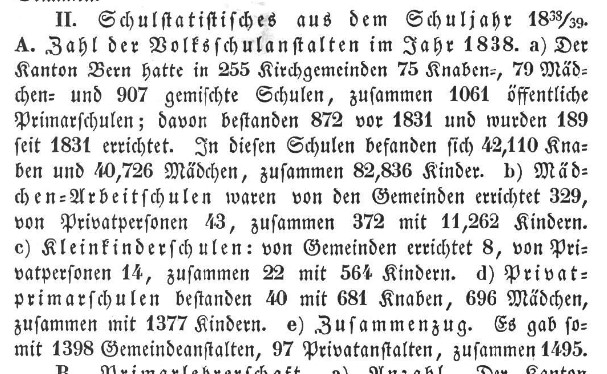
\includegraphics[width=0.7\textwidth]{../Figures/ass-001_1840_006_349_358_e739.jpg}
    \caption{Schulstatistik des Kantons Bern 1838/39 aus~\cite[356]{noauthor_kanton_1840}.}
    \label{figure:5-2}
\end{figure}

Die Statistik macht so sichtbar, wie viele Primarschulen im Kanton bestanden und wie viele männliche und weibliche Schüler*innen diese besuchten. Darüber hinaus bestand offensichtlich ein Interesse an öffentlichen Gemeindeschulen und wie viele seit 1831, dem Erlassjahr einer neuen liberalen Kantonsverfassung, gegründet wurden. Sie verschaffte also den Diskursteilnehmer*innen einen Überblick über die Expansion der öffentlichen Primarschule, einem zentralen Anliegen der liberalen Bewegung.

\pagebreak

Demgegenüber zeigt ein Beleg aus dem Kanton Thurgau gegen Ende des Untersuchungszeitraums eine deutlich komplexere Übersicht (Abbildung~\ref{figure:5-3}). Erhoben wird eine Reihe soziodemografischer Merkmale, anhand derer die Schüler*innen unterschieden werden:

\begin{itemize}
    \item Geschlecht
    \item Konfession
    \item geografische Herkunft (aus dem Schulort, bis 1 Stunde entfernt, mehr als 1 Stunde entfernt)
    \item Berufsstand der Eltern
    \item Schulbesuch
\end{itemize}

So entsteht ein Bild nicht nur über die thurgauischen Sekundarschüler*innen, sondern auch über ihre soziale Herkunft und welche Kategorisierungen zur gesellschaftlichen Selbstbeschreibung herangezogen werden: Die Unterscheidung zwischen männlichen und weiblichen Schüler*innen war bereits 1840 relevant und ist es immer noch. Daneben werden die Schüler*innen kategorisiert nach Religion (reformiert, katholisch, jüdisch) und Wohnort (Stadt, Umland, Land). Besonders interessant ist die Unterteilung der Schüler*innen nach dem elterlichen Beruf («Landwirthe», «Handwerker», «Handwerker mit Landwirthschaft», «Handelsleute», «Fabrikanten», «Beamte», «Lehrer», «Arme»). Hier zeigt sich, wie die Vielfalt der Berufe auf übersichtliche Kategorien eingegrenzt wird und der Beruf --- und nur ein Beruf pro Person --- zu einem Identitätsmerkmal wird. Dass es nicht unüblich war, mehrere Tätigkeiten auszuüben (vgl.~\cite[199]{vanderstraeten_soziale_2006}), schimmert noch in der Angabe «Handwerkern mit Landwirthschaft» durch, aber die Kategorienbildung ist schon weit fortgeschritten. Ebenso muss auch der erfasst werden, dessen Eltern keinen festen Beruf haben, hier in der Kategorie «Arm».

\begin{figure}[!ht]
    \centering
    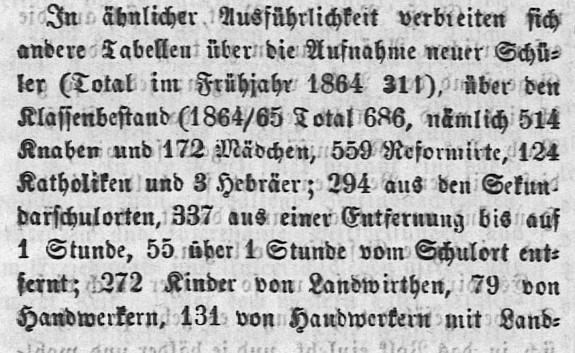
\includegraphics[width=0.7\textwidth]{Figures/slz-002_1866_011_25_32_e6.jpg}
    \caption{Sekundarschulstatistik Thurgau 1864/65 aus~\cite[24]{noauthor_schulnachrichten_1866}.}
    \label{figure:5-3}
\end{figure}

\section{Was Statistiken machen}\label{chapter5-3}

Im Rahmen des induktiven Vorgehens wurden die Lemmata \textit{Tabelle, Durchschnitt, Prozent} und \textit{Statistik} identifiziert, deren zunehmende Frequenz in unserem Korpus als Indiz für eine Zunahme statistischer Denk- und Redeweisen im Verlauf des 19.~Jahrhunderts gelesen werden kann. Die blosse Zunahme dieser Ausdrücke ist aber im Zusammenhang mit der Fragestellung noch wenig aussagekräftig. Zwar haben die Komposita im Zusammenhang der Grundformen bereits gewisse Aufschlüsse über Verwendungsformen von Tabellen und Statistiken geliefert, aber für eine umfassendere Analyse bietet es sich an, die Kollokationsprofile zu analysieren. Kollokationen sind statistisch signifikante Wortpaare oder Wörter, die in Nachbarschaft zu einander auftreten (siehe~\ref{Kollokationen}).

Interessant für eine weitergehende Analyse ist etwa Treffer 25 aus der KWIC-Ansicht zu \texttt{[word=\-\string"Sta\-ti\-stik"\-\%c]}: «Wie noch in vielen andern Sachen, herrscht gegenwärtig in den Schulen unseres Kantons ein wahres Wirrwar. Die Statistik der verschiedenen Lehrmittel beweist dies» (\cite[14]{noauthor_korrespondenzen_1858}). Aus sprachlicher Sicht interessant ist hier, dass einer Statistik ein handelnder Charakter zugesprochen wird, im obigen Beispiel «beweist» sie etwas. Aus wissenssoziologischer Perspektive lässt sich das als ein Akt der Konstruktion einer Tatsache lesen. Wie Heintz schreibt, werden hier «Zahlen […] nicht als selektive Beschreibungen einer zugrunde liegenden Wirklichkeit angesehen, sondern mit dieser selbst gleichgesetzt» (\cite[74]{heintz_zahlen_2007}). Wie äussert sich dies auf sprachlicher Ebene? Dazu wurden zu den Termini \texttt{.*tabell.*} und \texttt{.*statist.*} ein Kollokationsprofil von Token erstellt, die im Abstand von bis zu fünf Token rechts oder links der Suchbegriffe stehen. Die Kollokationen wurden anschliessend nach finiten Vollverben gefiltert. Angesichts der sehr problematischen Datenqualität sind die annotierten Daten aber nur mit Vorbehalt zu lesen.

\pagebreak

Die Treffer wurden nach dem «Log-likelihood»-Wert sortiert. Dieser ist ein Mass für die statistische Signifikanz einer Verbindung: Je höher der Log-likelihood-Wert für ein Token-Paar ist, desto eher können wir davon ausgehen, dass beide Token nicht zufällig miteinander auftauchen (\cite[139-147]{bubenhofer_sprachgebrauchsmuster_2009}). Wir erhalten eine Tabelle (\ref{table:5-1}) mit 27 Treffern.

\hspace{1cm}

\begin{longtable}{llrr}
    \toprule
    \textbf{Position} & \textbf{Token} & \textbf{Anzahl Kollokationen} & \textbf{Log-likelihood} \\
    \midrule
    \endfirsthead
    \multicolumn{4}{c}%
    {{\tablename\ \thetable{} -- Fortsetzung von vorheriger Seite}} \\[1mm]
    \textbf{Position} & \textbf{Token} & \textbf{Anzahl} & \textbf{Log-likelihood} \\
    \midrule
    \endhead

    \midrule \multicolumn{3}{r}{{Fortsetzung auf nächster Seite}} \\
    \endfoot

    \endlastfoot

    1 & enthält & 21 & 136.72 \\ 
    2 & nähern & 5 & 71 \\ 
    3 & ergibt & 13 & 49.05 \\ 
    4 & entnehmen & 10 & 47.514 \\ 
    5 & Fügen & 6 & 44.588 \\ 
    6 & zahlt & 8 & 29.178 \\ 
    7 & weist & 7 & 23.625 \\ 
    8 & zeigt & 14 & 19.798 \\ 
    9 & ergiebt & 5 & 15.57 \\ 
    10 & läßt & 7 & 14.953 \\ 
    11 & geben & 21 & 13.747 \\ 
    12 & folgen & 12 & 11.741 \\ 
    13 & u & 40 & 11.277 \\ 
    14 & ließ & 5 & 11.251 \\ 
    15 & od & 6 & 9.616 \\ 
    16 & besitzen & 6 & 8.255 \\ 
    17 & liefert & 5 & 7.873 \\ 
    18 & weisen & 5 & 7.565 \\ 
    19 & gaben & 5 & 3.353 \\ 
    20 & geht & 9 & 3.148 \\ 
    21 & gibt & 9 & 2.341 \\ 
    22 & zeigen & 5 & 2.171 \\ 
    23 & giebt & 6 & 1.564 \\ 
    24 & lassen & 10 & -0.029 \\ 
    25 & steht & 5 & -0.544 \\ 
    26 & macht & 5 & -1.254 \\ 
    27 & d & 6 & -8.463 \\ 
            \bottomrule
        \caption{Kollokationen zu \texttt{[word=".*ta\-bell.*|\-.*sta\-tist.*"]} gefiltert nach finiten Vollverben (\texttt{[pos="VVFIN"]})}
       \label{table:5-1}
    \end{longtable}

Das Kollokationsprofil ergibt, dass vor allem Verben des Zeigens und Beweisens statistisch überzufällig häufig mit Tabellen und Statistiken korrellieren. Unter den 23 Verben mit einem positiven Log-likelihood-Wert sind allein fünfzehn, die sich diesem Wortfeld zuordnen lassen oder auf Substantive wie \textit{Aufschluss} oder \textit{Hinweis} verweisen (\textit{enthält, ergibt, entnehmen, weist, zeigt, ergiebt, läßt, geben, folgen, liefert, weisen, gaben, geht, gibt, zeigen, giebt}). \textit{Geht} an Position 20 bezieht sich häufig auf «hervor».

\hspace{1cm}

    {\footnotesize
    \begin{spacing}{1}
    \renewcommand*{\arraystretch}{1.1}
    \begin{longtable}{p{0.1cm}p{5cm}p{1cm}p{5cm}}
        \toprule
        \textbf{Position} & \textbf{Kontext vor} & \textbf{Suchbegriff} & \textbf{Kontext nach} \\
        \midrule
        \endfirsthead
        \multicolumn{4}{c}%
        {{\normalsize \tablename\ \thetable{} -- Fortsetzung von vorheriger Seite}} \\[1mm]
        \textbf{Position} & \textbf{Kontext vor} & \textbf{Suchbegriff} & \textbf{Kontext nach} \\
        \midrule
        \endhead
    
        \midrule \multicolumn{4}{r}{{\normalsize Fortsetzung auf nächster Seite}} \\
        \endfoot
    
        \endlastfoot
            2 & Schenken wir darum schließlich auch diesem Falle noch unsere Aufmerksamkeit ! Unsere  & Schul\-statistik & \textbf{zeigt} allerdings , daß verhältnißmäßig mehr Lehrer ihren Stand wechseln , als  \\ 
            4 & zu genügen . Und in der That , ein Blick ans die & Zensur\-tabellen & \textbf{zeigt} , daß die Schulen um die Stadt herum fast alle nur   \\ 
            7 & im hiesigen Cantone unmittelbar vor der Einführung des nencn Schulgesetzes \textbf{zeigt} in & statistischer & Hinsicht die auf Beilage Nr. VI. befindliche , vom Erzichungsdepartemente damals veranstaltete \\ 
            8 & mehrere Präsidenten dieser Behörden aus . An mehrern Orten , mie die  & Vericht\-erstattungs\-tabelle & \textbf{zeigt} , steht es mit Rücksicht auf den Schulbesuch der Schulpflegen noch   \\ 
            9 & Real-Abtheilung zusammen 264 , und gegenwärtig 384 Schüler ; die Zusammenstellung der & Jahrestabellen & 	
            seit 1856 \textbf{zeigt} , einige Schwankungen abgerechnet , eine stetige Zunahme der   \\ 
            10 & Gemeinden wenig Er » freuliches berichtet werden . In Starkenbach zeigt die & Absenzen\-tabelle & auf einen Schüler durchschnittlich 9Ve , in Wintersberg 12 und in Ennetbühl   \\ 
            \bottomrule
        \caption{KWIC-Ansicht für \textit{zeigt} im Zusammenhang mit \texttt{[word=".*ta\-bell.*|\-.*sta\-tist.*"]}}
        \label{table:5-2}
    \end{longtable}
\end{spacing}}

Die Treffer der KWIC-Ansicht für das Verb \textit{zeigen}, die im Zusammenhang mit Schule stehen (Tabelle~\ref{table:5-2}), behandeln Unterschiedliches, etwa die Erwerbsbiografien des Lehrpersonals (Pos.~2), einen Vergleich der Schulqualität anhand der Noten (Pos.~4), die quantitative Entwicklung der Schülerzahlen (Pos.~10) oder die Entwicklung der Schulabsenzen (Pos.~11). Gemeinsam ist den Treffern, dass Statistik etwas sichtbar macht, was ohne sie nicht sichtbar wäre und nun mit einem einfachen finiten Verb als Beweis in den Diskurs eingeführt werden kann. 

\begin{figure}[!ht]
    \centering
    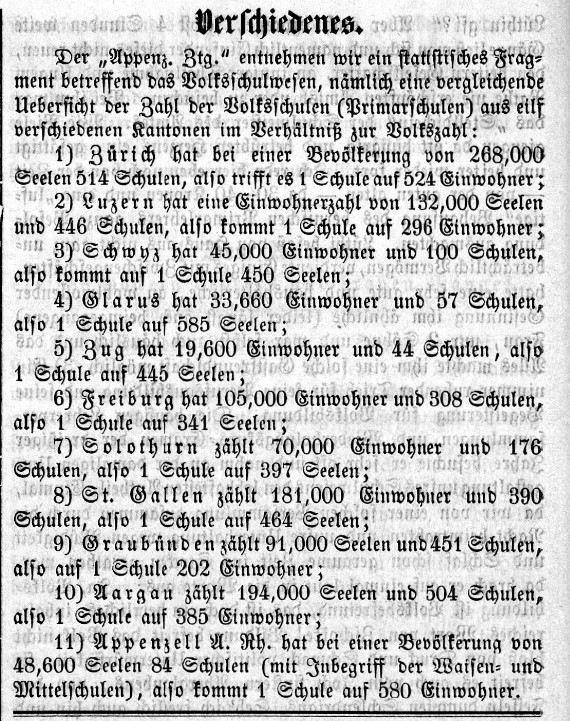
\includegraphics[width=0.65\textwidth]{Figures/bso-001_1864_007_141_144_e38_s144.jpg}
    \caption{Auszug aus~\cite{noauthor_verschiedenes_1864}.}
    \label{figure:5-4}
\end{figure}

Entgegen der ursprünglichen Erwartung finden sich in den Treffern kaum Belege dafür, dass Kategorien der gesellschaftlichen Selbstbeschreibung kombiniert werden. Am häufigsten zu finden sind Aufstellungen der Zahl der Schulen, der Schülerinnen und Schüler und besonders der Absenzen. Die Angaben zur Zahl der Schulen sind recht summarisch gehalten und nennen in der Regel nur Orte. Das Beispiel in Abbildung~\ref{figure:5-4} kommt einer anfänglich erwarteten Konstruktion der schweizerischen Gesellschaft durch Statistiken noch am nächsten. Hier wird die Anzahl der Schulen pro Einwohner für einige Kantone verglichen. Ein Versuch, daraus beispielsweise zu argumentieren, dass katholische Kantone sich in Bezug auf die Schulbildung von reformierten Kantonen unterschieden, wird hingegen nicht unternommen.

\pagebreak

\section{Wie Statistiken Kontrolle ausüben}\label{chapter-5-4}

Was die Statistiken und Tabellen aus Kapitel~\ref{chapter5-3} häufig «zeigen» oder worüber sie Aufschluss geben, sind die Absenzen der Schüler*innen. Die Tabelle und die Statistik als Kontrollinstrument staatlicher Macht ist ein klassisches Thema der Statistikgeschichte. Die Erfassung von deviantem Verhalten in Form von Suizid- oder Kriminalstatistiken machte einen grossen Teil der Flut an Statistiken ab 1830 aus (\cite[30]{porter_rise_1986}). Auch im vorliegenden Korpus spielt die Erfassung von Normabweichungen eine grosse Rolle. So sollten mit statistischen Erhebungen Schüler*innen und Lehrer*innen überwacht werden, um Probleme zu identifizieren und behandeln zu können (\cite[217]{ruoss_zahlen_2018}).

Bis 1858 hatten alle Kantone eine allgemeine Schulpflicht für den Primarschulbesuch eingeführt. Deren Durchsetzung war das ganze 19.~Jahrhundert hindurch indes umstritten. Die Arbeitskraft der Kinder war vielerorts wirtschaftlich notwendig, gerade im Sommer in der Landwirtschaft. Daneben wurde die Schule auch als Ort (kantonal-)staatlicher Normierungsversuche wahrgenommen, sodass Eltern ihre Kinder nicht auf die Schulen schicken wollten. Dagegen versuchten die Schulverwaltungen die Schulpflicht durchzusetzen (\cite[26-27]{criblez_einleitung_1999}). Wie bereits in Kapitel~\ref{chapter4-2-2-1} angedeutet, spielten Statistiken und Tabellen dabei eine wichtige Rolle. Einige Treffer im Kontext des Suchbegriffs \texttt{[word\-=".*tabell.*"} betreffen das Thema der Schulabsenzen. Diese sind in Tabelle~\ref{table:5-3} dargestellt.

\hspace{1cm}

\renewcommand{\arraystretch}{1}{
\begin{table}[!ht]
    \centering
    \begin{tabular}{llr}
        \toprule
        \textbf{Position} & \textbf{Token} & \textbf{Anzahl} \\
        \midrule
        18 & Schultabellen & 12 \\ 
        22 & Versäumnißtabellen & 11 \\ 
        23 & Absenztabellen & 8 \\ 
        38 & Schultabelle & 5 \\ 
        \bottomrule
    \end{tabular}
    \caption{Auswahl aus Treffern für \texttt{[word=\-".*tabell.*"\%c]}}
\label{table:5-3}
\end{table}
}

Wenn wir die Suche auf Begriffe im Zusammenhang mit \textit{Versäumniß} und \textit{Absenz} ausdehnen, finden sich noch weitere Wörter, die die Funktion von \textit{-tabelle} einnehmen (\cref{table:5-4}).

\hspace{1cm}

\renewcommand{\arraystretch}{1}{
    \begin{table}[!ht]
        \centering
        \begin{tabular}{llr} \toprule
            \textbf{Position} & \textbf{Token} & \textbf{Anzahl} \\ \midrule 
            7 & Versäumnißtabellen & 11 \\
            10 & Absenzenverzeichnisse & 8 \\
            11 & Absenztabellen & 8 \\
            15 & Absenzenlisten & 4 \\
            16 & Absenzenverzeichniß & 4 \\
            21 & Absenzenlistcn & 3 \\
            22 & Absenzentabellen & 3 \\
            23 & Versäumnißrodel & 3 \\
            24 & Versäumnißtabelle & 3 \\
            25 & Absenzenliste & 2 \\
            37 & Absenzcnrapporte- & 1 \\
            38 & Absenzcntabellcn & 1 \\
            46 & Absenzen-Verzeichnisse & 1 \\
            47 & Absenzenberichten & 1 \\
            53 & Absenzenrgtster & 1 \\
            55 & Absenzenrodel & 1 \\
            56 & Absenzenrodels & 1 \\
            59 & Absenzentabelle & 1 \\
            \bottomrule
        \end{tabular}
        \caption{Auswahl aus Treffern für \texttt{[word=\-"Versäumniß.*|Absenz.*"]}}
        \label{table:5-4}
    \end{table}
}

Wir können daher die Begriffe \textit{-listen}, \textit{-verzeichnis}, \textit{-rodel}, \textit{-rapport} und \textit{-berichte} in die Suche aufnehmen. Ausserdem tauchen auch vom OCR falsch erkannte Token auf wie \textit{Absenzcn-} oder \textit{listcn}. Nehmen wir diese Begriffe in eine Suchanfrage auf, erhalten wir insgesamt 41 Belegstellen, die sich in Texten ab 1835 finden lassen. Aufgrund der insgesamt niedrigen Frequenz der Token sind die Balken in Abbildung~\ref{figure:5-5} mit Vorbehalt zu lesen. Dennoch lässt sich festhalten, dass die Praxis der Dokumentation von Schulabsenzen in Tabellen, Listen oder ähnlichen Verzeichnissen einen Niederschlag auf der Textoberfläche findet.

\begin{figure}[!ht]
    \begin{tikzpicture}    
    \pgfplotstableread[col sep=comma]{./Data/abbildung-5-5-absenzenlisten.csv}{\loadedtable}
    \begin{axis}[
        ybar,
        width=\linewidth,
        ymajorgrids=true,
        xlabel=Jahr,
        ylabel=Treffer per Mio.~Wörter,
        legend style={at={(xticklabel cs:.5)},anchor=north},% Legende abhänging von xticks positioniert
        x tick label style={rotate=90,anchor=east},
        xmin = 1799,
        xmax = 1871,
        height = 5cm,
        bar width=3pt,
        xtick pos = left,
        ytick pos = left,
        ymin = 0,
      ]
    \addplot[x=Jahr, y=Treffer per Mio. Wörter, color=zhawgray, fill]table{\loadedtable};
    \end{axis} 
    \end{tikzpicture}  
    \caption{Relative Häufigkeiten für \texttt{[word=\string"\phantom{}Ab\-senz\-ta\-bellen|\-Abs\-enz\-en\-li\-sten|\-Ab\-senz\-en\-ver\-zeich\-niß|Absenz\-en\-ver\-zeic\-hnisse|\-Ab\-senz\-en\-list\-cn|\-Ab\-sen\-zen\-tab\-el\-len|\-Ver\-säum\-niß\-ro\-del|\-Ver\-säum\-niß\-ta\-belle|\-Ab\-senz\-en\-lis\-te|\-Ab\-senz\-cn\-rapporte|\-Ab\-senz\-en-Ver\-zeich\-nisse|\-Ab\-senz\-en\-be\-rich\-ten|\-Schul\-listen|\-Schul\-ta\-bellen|\-Ver\-säum\-niß\-ta\-bellen"]}}
    \label{figure:5-5}
\end{figure}

Mit den Absenzenlisten sollte die Einhaltung der in vielen Gegenden noch ungewohnten gesetzlichen Schulpflicht durchgesetzt und kontrolliert werden. Dem Lehrpersonal wurde aufgetragen, die Listen genau zu führen und regelmässig zum Bericht einzusenden, wie etwa das Beispiel aus Appenzell Ausserrhoden zeigt: «Allein an einer richtigen und genauen Tabellenführung und konsequenten Bestrafung der Schulversäumnisse liegt viel mehr, als es den Anschein hat. Es klingt paradox und ist doch buchstäbliche Wahrheit, daß die Schultabellen einen wesentlichen Einfluß auf die Hebung der Schulen in Außerrhoden ausgeübt haben, vorab auf einen regelmäßigen und fleißigen Schulbesuch; ja sie haben ganz allmälig den obligatorischen Schulzwang eingeführt» (\cite[68]{noauthor_neuesten_1868}). So wurde die Zahl der Absenzen zu einem Gradmesser für die Reichweite der Volksbildung und es liessen sich säumige Eltern, Lehrer und Schulgemeinden identifizieren (vgl.~Abbildung~\ref{figure:5-6}). Der Fortschritt der Bildungsexpansion wird also auf eine eindeutige, diskrete Zahl reduziert, welche Vergleiche ermöglicht, Muster aufzeigt und auf Steuerungsbedarf hinweist.

\pagebreak

\begin{figure}[!ht]
    \centering
    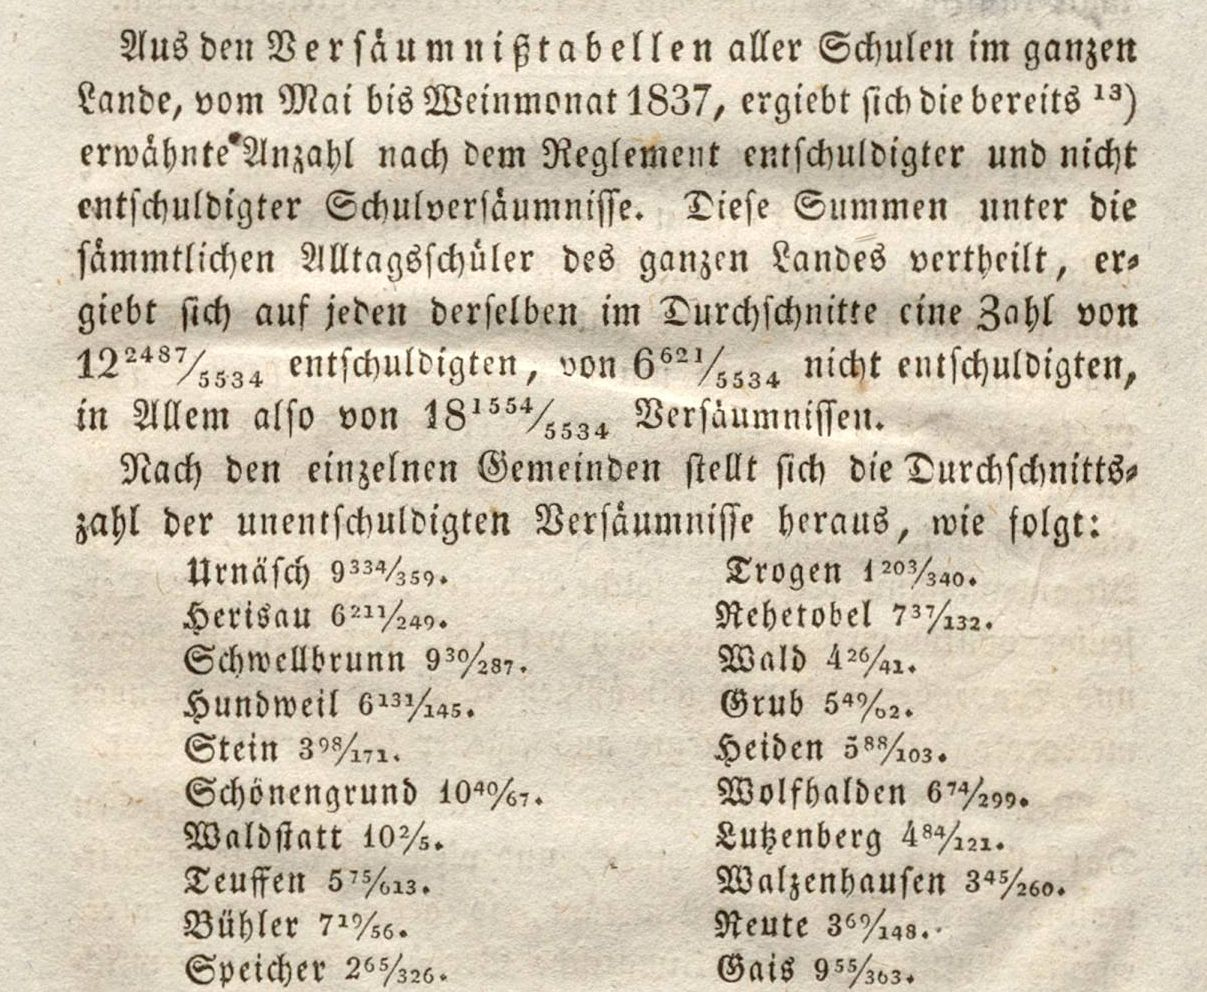
\includegraphics{../Figures/absenzen-apm-001_1838_014_0035.jpg}
    \caption{Schulabsenzen in Appenzell 1837 aus~\cite[29]{noauthor_nachlese_1838}.}
    \label{figure:5-6}
\end{figure}

\begin{figure}[!ht]
    \begin{tikzpicture}    
    \pgfplotstableread[col sep=comma]{./Data/abbildung-5-7-absenzen.csv}{\loadedtable}
    \begin{axis}[
        ybar,
        width=\linewidth,
        ymajorgrids=true,
        xlabel=Jahr,
        ylabel=Treffer per Mio.~Wörter,
        legend style={at={(xticklabel cs:.5)},anchor=north},% Legende abhänging von xticks positioniert
        x tick label style={rotate=90,anchor=east},
        xmin = 1799,
        xmax = 1871,
        height = 7cm,
        bar width=3pt,
        xtick pos = left,
        ytick pos = left,
        ymin = 0,
      ]
    \addplot[x=Jahr, y=Treffer per Mio. Wörter, color=zhawgray, fill]table{\loadedtable};
    \end{axis} 
    \end{tikzpicture}  
    \caption{Relative Häufigkeiten für \texttt{[word=\string"\phantom{}Ab\-senz.*|Versäum\-niß"\%cd]}}
    \label{figure:5-7}
\end{figure}

Angesichts der geringen relativen Häufigkeit der Treffer zu den Absenztabellen wurde zusätzlich nach den Token, die mit \textit{Absenz} oder \textit{Versäumniß} anfangen, gesucht. Diese treten ab 1834 auf (Abbildung~\ref{figure:5-7}).\footnote{Alle Treffer vor 1834 behandeln nicht Schulabsenzen.}  Der erste Treffer ist ein 1834 Antrag des Schulkapitels Bülach bei der Zürcher Schulsynode: «Der hohe Regierungsrath möchte durch kräftige Maaßregeln (sic!) […] den zahlreichen Absenzen Abhilfe verschaffen zu suchen» (\cite[30]{noauthor_general-bericht_1834}, zur Zürcher Schulsynode siehe~\cite{trohler_zurcher_2007}). Ab diesem Zeitpunkt sind die beiden Zeichenfolgen \textit{Absenz} und \textit{Veräumniß}, mit gewissen Konjunkturen, fast durchgängig im Korpus vertreten. Der Ausschlag für das Jahr 1849 in Abbildung~\ref{figure:5-7} erklärt sich mit einer geringeren Menge an Texten im Korpus mit diesem Erscheinungsjahr, sodass die relative Häufigkeit deutlich ansteigt. 

\begin{figure}[!ht]
    \centering
    \includegraphics[width=0.8\textwidth]{./Figures/bso-001_1864_007_0184.jpg}
    \caption{Schulabsenzen im Oberaargau 1864 aus~\cite[184]{noauthor_bernische_1864}.}
    \label{figure:5-8}
\end{figure}

\pagebreak

Im Jahr 1864 sorgt ein mehrteiliger Aufsatz in der «Neuen Berner Schul-Zeitung», «Die bernische Volksschule auf der Anklagebank», für einen weiteren deutlichen Peak. Es ist eine bernische Entgegnung auf einen kritischen Artikel in der «Schweizerischen Lehrerzeitung» zum mangelnden Zustand der Schulen im Kanton Bern, der besonders an den vielen Absenzen festgemacht wurde. Herzstück der Replik ist eine umfassende Tabelle der Schulabsenzen im Oberaargau, aufgeteilt nach Ämtern. Angegeben werden die Absenzen der Schüler nach Ort, Klassenstufe und die Zahl der Absenzen. Als signifikantes Muster werden die Unterschiede der Absenzen im Sommer und Winter ausgemacht (Abbildung~\ref{figure:5-8}). 

Wie Abbildung~\ref{figure:5-6} tragen solche Statistiken zum «Nation Building» des Kantons Bern bei, wenn sie die Gemeinde- und Bezirkszugehörigkeiten im Diskurs reifizieren. Allerdings werden keine Bezüge zwischen den Ämtern oder Orten und ihrer Sozialstruktur hergestellt. Höchstens im Subtext lässt sich die Botschaft identifizieren, dass Bern im Vergleich mit dem Kanton Zürich nicht rückständig ist. Auffällig im Vergleich zu Abbildung~\ref{figure:5-6} ist die Darstellungsform, die sich deutlich in Richtung von statistischen Tabellen bewegt. Noch deutlicher wird diese im Beispiel des Kantons Zürich. Sie zeigt auch die fortschreitende Kategorisierung der Absenzen, die nach verantwortbaren Absenzen, etwa durch Krankheit, und strafbare Absenzen eingeteilt werden. Es werden Durchschnitte pro Schüler berechnet und nach Bezirken aufgestellt, was einen Vergleich der Bezirke erlaubt. Warum aber die Absenzenzahlen im Schuljahr 1857/58 in Zürich 15.02, in Winterthur aber nur 9.26 betragen, wird im Begleittext nicht erklärt (Abbildung~\ref{figure:5-9}).

\begin{figure}[!ht]
    \centering
    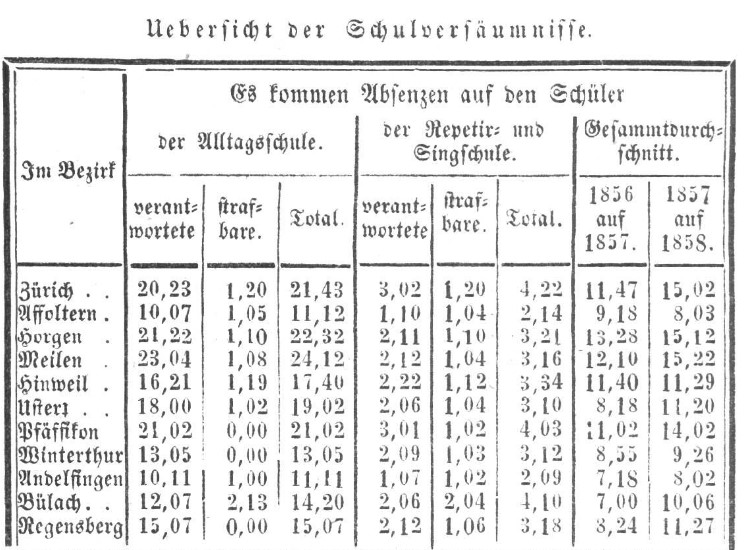
\includegraphics[width=0.7\textwidth]{./Figures/syn_001_1858_000_22_60_e105_24.jpg}
    \caption{Schulabsenzen im Kanton Zürich 1856–1858 aus~\cite[24]{noauthor_jahresbericht_1858}.}
    \label{figure:5-9}
\end{figure}

Unter den Treffern zu den Absenzen finden sich nun einige, die die Absenzenzahlen mit soziodemografischen Mustern in Verbindung bringen, so etwa ein Bericht des Waadtländer Staatsrates zu den Schulen im Jahr 1856. Für den Bezirk Orbe werden die sozio-ökonomischen Unterschiede zwischen den Orten im Jura und denen der Ebene als Gründe für Unterschiede der Schulabsenzen angeführt: 

\begin{displayquote}
in den Bergen ist er [der Schulbesuch, M.~K.] viel besser als in der Ebene; hier halten die ländlichen Arbeiten die Kinder oft von der Schule ab. Ferner ist der Geschmack am Unterricht in der Ebene weniger entwickelt als in den Bergen; das erklärt zum Theil die häufigern Absenzen in dem Landestheile, welcher am Fuße des Jura liegt (\cite[287]{noauthor_mittheilungen_1858}).
\end{displayquote}

Für den Bezirk Yverdon heisst es an gleicher Stelle: 

\begin{displayquote}
Was den Schulbesuch betrifft, so ist ein merkbarer Unterschied zwischen der Stadt und dem Lande. In der ersteren sind die Absenzen und Disciplinarfälle zahlreicher als in den Landgemeinden durch Schuld der Eltern, welche ihre Kinder unter den kleinlichsten Verwänden zurückhalten und sie durch ihr Beispiel und ihre Reden zur Mißachtung der Lehrer anleiten. In den Dörfern im Gegentheil, und besonders in denjenigen, wo ein gewisser Wohlstand herrscht, bemerkt man am Fleiße und an der Gelehrigkeit der Kinder leicht, daß die Eltern den Werth des Unterrichts und einer guten religiösen Erziehung schätzen. Davon sind auszunehmen die armen Gemeinden, wo die Gewohnheiten der Trunkenheit, des Nichtsthuns, des Bettelns das tägliche Leben vieler Familien geworden sind und auf eine traurige Weise auch die Schuljugend anstecken (\cite[287]{noauthor_mittheilungen_1858}).
\end{displayquote}

Durch die Schulstatistik und besonders die Absenzen wird ein sozio-demografisches Bild des Bezirks gezeichnet. Interessanterweise ist es die Stadt, in der die Rückständigkeit beklagt wird. Dagegen wird die Landbevölkerung als bildungsfleissig dargestellt. Scharf von letzterer ausgenommen werden jedoch die armen Gemeinden. Hier werden Bildungsfleiss und ökonomische Lage verknüpft. Für den Waadtländer Staatsrat scheint es klar zu sein, dass arme Familien auch bildungsferne Familien sind.

Andererseits zeigen die Belege auch die Schwierigkeiten im Umgang mit der Statistik als Überwachunstechnologie. Zahlreich werden nachlässig geführte Listen beklagt oder Lehrer verweisen auf die Kompliziertheit und die Mühen des Ausfüllens der Formulare. Der «avalanche of numbers» erzeugte nicht nur Ordnung erzeugt, sondern auch ein zu viel an Daten. Zudem war auch den Zeitgenossen bewusst, dass hinter den scheinbar eindeutigen Zahlen oft zweifelhafte Erhebungspraktiken standen. Dies ist ebenfalls ein Befund der kritischen Statistikgeschichte (nur ein Beispiel:~\cite[88]{bruckweh_menschen_2015}). Entsprechend finden sich auch im Korpus Belege, die den Wert einer auf Zahlen reduzierten Messung der Schulqualität anzweifeln: 

\begin{displayquote}So wie sich aber diese Kontrolle fast ausschließlich nur auf die Absenztabellen beschränkte, so eben auch der Jahresbericht, und man gab sich so ziemlich dem Glauben hin, als seien die Absenztabellen der sicherste Maßstab zur Beurtheilung des Zustandes der Schulen (\cite[272]{noauthor_schulvisitationen_1855}).
\end{displayquote}

\section{Kontrollüberschuss von Statistiken}
Das Interessante an der Entbergung latenter Muster anhand statistischer Daten ist, dass Daten stets mehr verraten können als den Zweck, für den sie erhoben werden. Dafür sorgt die ihre «radikale Rekombinationsfähigkeit» (\cite[128]{nassehi_muster_2019}). Auf Zahlen reduzierte soziale Phänomene sind frei kombinierbar. Sie können ausserhalb ihres Verwendungskontextes eingesetzt und mit anderen Zahlen in Bezug gesetzt werden: Daten werden verknüpft und neue Einsichten in gesellschaftliche Muster sind im Diskurs formulierbar. Auch dieses Phänomen findet sich im vorliegenden Korpus im Fall von Statistiken. So behandelte ein anonymer Autor in der «Neuen Berner Schulzeitung» 1865 die Frage «Ist die physische Entartung der jetzigen Generation eine Thatsache?» und kombinierte in seiner Problemanalyse medizinische und Schulstatistiken: 

\begin{displayquote}
    Ueber den nachtheiligen Einfluß unzweckmäßiger Einrichtungen geben uns den sichersten Aufschluß die Journale der Aerzte, die Todtenlisten und die Zahl der stets auf betrübende Weise zunehmenden Fälle von Rückgratskrümmungen, Brustkrankheiten, Kopfschmerzen und Augenleiden unserer Schuljugend und unsere daher rührenden Absenzenverzeichnisse (\cite[70]{j_erste_1865}).
\end{displayquote}

Auf sprachlicher Ebene äussert sich dies in diesem Zitat in einer Aufzählung verschiedener Arten von Listen, deren Kombination «Aufschluß gibt», und zwar über die baulichen Zustände der Schulhäuser. Das ist etwas völlig anderes als das, wofür die Absenzenverzeichnisse, Medizinalstatistiken und Mortalitätslisten ursprünglich erstellt worden waren.

Den Statistiken ist also ein «Kontrollüberschuss» (Dirk Baecker, zit.~n.~\cite[43-44]{nassehi_muster_2019}). Durch ihre Rekombinationsfähigkeit enthalten Daten stets ein mehr Informationen, dass sich für Rückschlüsse auf Regelungsbedürftiges nutzen lässt. Ein Beispiel aus dem Korpus ist dafür Treffer 10 in Tabelle~\ref{table:5-2}. Darin kommentiert der Autor den Amtsbericht des evangelischen Erziehungsrats des Kantons St.~Gallen für das Jahr 1855. Die in der Statistik enthaltenen Zahlen werden als Fakten zitiert, denen eine Beweisfunktion zukommt. Auf dieser Grundlage schliesst der Kommentator, die auf tiefgehende Missstände im Umkreis der Schule:

\begin{displayquote}
    «In Starkenbach zeigt die Absenzentabelle auf einen Schüler durchschnittlich 9½, in Wintersberg 12 und in Ennetbühl 17 unentschuldigte Abwesenheiten.» Wo solche Krebsschäden sich zeigen, da suche man die Ursache nicht an einem Orte, und erinnere herzhaft nicht nur die Eltern, sondern auch Lehrer und Schulräthe an ihre Pflichten. Nur radikales Einschreiten kann da helfen, wo Nachläßigkeit und Gleichgültigkeit das Schulleben anzugreifen drohen (\cite{sch_mittheilungen_1856}).
\end{displayquote}

Hier wird von den diskursiv eingeführten Zahlen auf gesellschaftliche Zustände geschlossen. Die Statistik erweist sich nicht nur als Kontrollmittel der Schülerinnen und Schüler sowie ihrer Eltern, sondern auch von Amtspersonen wie den Schulräten. Die Tabellen entdecken nicht nur ein Muster im Absenzverhalten der Schülerinnen, sondern vielmehr Nachlässigkeiten im Disziplinierungsapparat. Sie sind ein Mittel der «Biopolitik». Es wird nicht gemessen, um zu wissen, sondern um andere zu einem erwünschten Verhalten zu disziplinieren. Eine solche datengestützte Form der Disziplinierung ist nur möglich in einer Gesellschaft, die digital sehen gelernt hat, ergo digitalisiert ist (\cite[309-310]{nassehi_muster_2019}).  

\section{Zwischenfazit}
Statistiken im Schweizer Schuldiskurs des 19.~Jahrhunderts zählten Schüler*innen vor allem nach Schulort und Geschlecht. Festgestellt wurde auch eine zunehmend komplexere Kategorisierung, die weitere Kategorien erhob. Allerdings konnte im Korpus weder eine klare Tendenz dahingehend festgestellt werden, dass die Erhebung dieser zusätzlichen Kategorien weiter verbreitet gewesen wäre. Auch Belege zu einer expliziten Kombination der Schüler*innenzahlen wurden kaum gefunden. Was die Statistiken im Diskurs «zeigen», wenn auf sie sprachlich verwiesen wurde, sind meist eben die Zahlen zur Anzahl nach Ort aufgeschlüsselt.

Anhand der Schulabsenzen konnten dagegen Belege gefunden werden, die die Hypothesen dieser Arbeit stützen. Es konnte gezeigt werden, dass die Statistiken und Tabellen eine Überwachungs- und Kontrollfunktion innehatten. Diese erstreckte sich nicht nur auf die Schüler*innen und ihre Eltern, sondern auch auf Lehrer und die Schulgemeinden. 
%% Indicate the main file. Must go at the beginning of the file.
% !TEX root = ../main.tex

%----------------------------------------------------------------------------------------
% CHAPTER TEMPLATE
%----------------------------------------------------------------------------------------


\chapter{Diskussion} % Main chapter title

\label{Chapter6} % Change X to a consecutive number; for referencing this chapter elsewhere, use \ref{ChapterX}

%----------------------------------------------------------------------------------------
% SECTION 1
%----------------------------------------------------------------------------------------

\section{Digitalisierung der Schweizer Gesellschaft}

Lorem ipsum dolor sit amet, consectetur adipiscing elit. Aliquam ultricies lacinia euismod. Nam tempus risus in dolor rhoncus in interdum enim tincidunt. Donec vel nunc neque. In condimentum ullamcorper quam non consequat. Fusce sagittis tempor feugiat. Fusce magna erat, molestie eu convallis ut, tempus sed arcu. Quisque molestie, ante a tincidunt ullamcorper, sapien enim dignissim lacus, in semper nibh erat lobortis purus. Integer dapibus ligula ac risus convallis pellentesque.

%-----------------------------------
% SUBSECTION 1
%-----------------------------------
\subsection{Bildung gesellschaftlicher Kategorien}

Nunc posuere quam at lectus tristique eu ultrices augue venenatis. Vestibulum ante ipsum primis in faucibus orci luctus et ultrices posuere cubilia Curae; Aliquam erat volutpat. Vivamus sodales tortor eget quam adipiscing in vulputate ante ullamcorper. Sed eros ante, lacinia et sollicitudin et, aliquam sit amet augue. In hac habitasse platea dictumst.

%-----------------------------------
% SUBSECTION 2
%-----------------------------------

\subsection{Problematisierung anhand von Statistiken}
Morbi rutrum odio eget arcu adipiscing sodales. Aenean et purus a est pulvinar pellentesque. Cras in elit neque, quis varius elit. Phasellus fringilla, nibh eu tempus venenatis, dolor elit posuere quam, quis adipiscing urna leo nec orci. Sed nec nulla auctor odio aliquet consequat. Ut nec nulla in ante ullamcorper aliquam at sed dolor. Phasellus fermentum magna in augue gravida cursus. Cras sed pretium lorem. Pellentesque eget ornare odio. Proin accumsan, massa viverra cursus pharetra, ipsum nisi lobortis velit, a malesuada dolor lorem eu nequ

%----------------------------------------------------------------------------------------
% SECTION 2
%----------------------------------------------------------------------------------------

\subsection{Kontrollüberschuss der digitalen Methoden}


\section{Zahlen erzählen: zum diskursiven Verweis auf Statistiken und Statistik als Argument}

\begin{itemize}
    \item\cite{espeland_narrating_2015} hat einen spannenden Ansatz dafür, dass Zahlen nicht für sich selber sprechen, sondern diskursiv zum Thema gemacht werden müssen, sie müssen in Narrative eingebettet werden
    \item Zahlen werden gemäss Heintz eingesetzt, «Argumente mit einer Aura des Notwendigen zu versehen»
    \item Zahlen, die empirische Fakten abbilden sollen, haben eine spezielle argumentative Qualität: sie erlauben, ähnlich wie Abbildungen, keine einfache Negation in Form eines "Ja/Neins", sondern ihre Herstellung muss problematisiert werden, das ist aufwändiger als die rein sprachliche Negation \cite[78]{heintz_zahlen_2007} 
    \item \cite{ruoss_zahlen_2018} hat dazu auch für den Fall der Schweizer Bildungsgeschichte etwas gemacht, sehr aufschlussreich, aber erst ab 1890
    \item Wir fragen hier, ob es auf der sprachlichen Oberfläche Hinweise gibt, wie Zahlen und Statistiken argumentativ eingesetzt werden. 
\end{itemize}

\begin{verbatim}
    [word ="zahl.*|.*statist.*"] []* [pos ="VVFIN"] within s
\end{verbatim}
% Indicate the main file. Must go at the beginning of the file.
% !TEX root = ../main.tex

%----------------------------------------------------------------------------------------
% CHAPTER TEMPLATE
%----------------------------------------------------------------------------------------


\chapter{Fazit} % Main chapter title

\label{Chapter7} % Change X to a consecutive number; for referencing this chapter elsewhere, use \ref{ChapterX}

%----------------------------------------------------------------------------------------
% SECTION 1
%----------------------------------------------------------------------------------------

\section{Die Digitalisierung der Schweizer Gesellschaft anhand des Schuldiskurses}

Ziel der Arbeit war es, den Diskurs um die Volksschule in der Schweiz im 19.~Jahrhundert mit korpuslinguistischen Methoden zu analysieren. Dabei sollte herausgearbeitet werden, wie Statistik auch in der Schweiz dazu beitrug, Vorstellungen von Gesellschaft möglich zu machen und wie sich dies diskursiv im vorliegenden Korpus niederschlug. Die Annahme war, dass wir deshalb bereits im 19.~Jahrhundert von einer Digitalisierung der Schweizer Gesellschaft sprechen können, die sich nur durch digitale Techniken beschreiben liess. Diese digitalen Techniken reduzierten die komplexe Gesellschaft der Individuen auf diskrete Zahlen und Kategorien und erlaubten es so, latente Verhaltensmuster sichtbar zu machen.

%-----------------------------------
% SUBSECTION 1
%-----------------------------------
\subsection{Statistikgeschichte}

Zunächst wurde in Kapitel~\ref{Fragestellung} gefragt, ob es beobachtbare Veränderungen auf der sprachlichen Oberfläche des Diskurses gibt, die auf eine zunehmende Bedeutung statistischer Redeweisen gibt. Die explorative Analyse in Kapitel~\ref{Chapter4} konnte nachweisen, dass sich im vorliegenden Korpus ab etwa 1830 zunehmend statistische Termini finden. Tabellen, Statistiken, Durchschnitte und Prozentangaben tauchen auf der sprachlichen Oberfläche des Diskurses auf. Am Wort \textit{Statistik} konnte gezeigt werden, dass es Kompositabildungen anregt. Im Diskurs tauchen Statistiken aller Art auf, etwa zu Schulen, zur Kriminalität oder zum Obstbau. Dass es möglich ist, solche Komposita zu bilden, illustriert, wie die statistische Selbstbeobachtung dazu führt, unterschiedliche Sozialbereiche und Themenfelder abzustecken.

%-----------------------------------
% SUBSECTION 2
%-----------------------------------

\subsection{Statistik im Schuldiskurs}

In Kapitel~\ref{Chapter5} konnten zuerst in Bezug auf Frage 3 gezeigt werden, in welche Gruppen Schüler*innen kategorisiert wurden und wie diese Kategorien als Repräsentation von Gesellschaft gelesen werden können. Es waren dies zunächst Geschlecht und regionale Kriterien wie die Aufteilung in Schulbezirke. Gegen Ende des Untersuchungszeitraums konnte an einem Beispiel eine zunehmende Komplexität belegt werden, die auch Religion und soziodemografischen Status des Vaters mit einbezog. 

Allerdings konnte kaum, wie von Frage 4 gefragt, nachgewiesen werden, dass diese Kategorien gesellschaftlicher Selbstbeschreibung häufig zueinander in Bezug gesetzt wurden. Schüler*innen\-zahl\-en wurden in Tabellen und Listen, meist nach Bezirk oder Ort, rapportiert, aber nur wenige Belege gefunden, wie diese Kategorien diskursiv verbunden wurden, um Muster sozialen Verhaltens zu belegen. Argumente wie beispielsweise «Die Statistik zeigt, dass katholische Kantone weniger Schulen besitzen und ärmer und weniger gebildet sind» wurden explizit nur selten gemacht.

Anhand von Statistiken und Tabellen zu den Schulabsenzen konnte deutlicher gezeigt werden, dass Techniken des «digitalen Sehens» im Schweizer Diskurs um die Schule etabliert waren. Hier konnten zentrale Annahmen bestätigt werden, etwa dass Statistiken dafür eingesetzt wurden, Muster des Verhaltens sichtbar zu machen und zu adressieren. Ausserdem wurde der den digitalen Techniken inhärente Kontrollüberschuss aufgezeigt. Durch die Rekombination der Daten wurde beispielsweise sichtbar gemacht, in welchen Orten die Schulabsenzen höher waren und dies mit der Sozialstruktur der betroffenen Gemeinden in Verbindung gebracht.

\subsection{Doch keine Digitalisierung im 19.~Jahrhundert?}

Die These einer Digitalisierung der Schweizer Gesellschaft zwischen 1830 und 1870 im Spiegel der Schulstatistik kann daher in Ansätzen bestätigt werden. Sie überzeugt vor allem für die allgemeine Entwicklung des Schulwesens und die Durchsetzung der allgemeinen Schulpflicht mittels Absenzenlisten. Mittels der Schul- und Schülerzahlen wurde der Fortschritt des Schulausbaus verfolgt und ansichtig gemacht. Kantonale Darstellungen zeigten, wie es um den regionalen Ausbau der Schulen stand, aber es wurden nur selten konkrete Zusammenhänge zwischen Sozialstruktur und Schulausbau formuliert.

Dies könnte darauf hinweisen, dass das Statistikwesen der Schweiz doch einen Nachzügler im europäischen Vergleich darstellt. Diese These wird von der bisherigen Forschung so vertreten und begründet mit der schwachen Position des Eidgenössischen Bureaus für Statistik gegenüber den Kantonen. Ruoss beispielsweise untersucht differenzierte Schulstatistiken ebenfalls erst ab 1890 (\cite{ruoss_zahlen_2018}). Um diese These genauer überprüfen zu können, müsste das Korpus auf Quellen nach 1870 ausgeweitet werden.

Ein weiterer Grund, weshalb die Hypothese nicht überzeugend bewiesen werden konnte, könnten die Korpusquellen sein. Genügen die im Korpus vertretenen Texte doch nicht für eine entsprechende Untersuchung oder müsste es erweitert werden? Die angewandten Suchtstrategien könnten ebenfalls im Lichte dieser Untersuchung optimiert werden. Es stehen weitere Ansätze der maschinellen Textanalyse zur Verfügung, die hier nicht angewendet wurden. Das gewählte Vorgehen war ausserdem einigermassen eklektisch. 

Ein gewichtiges Problem des Korpus stellt die problematische Datenqualität dar. Wie an mehreren Stellen gezeigt, sind die OCR-erkannten Texte mit vielen Fehlern behaftet, besonders die von Frakturschriften. Zahlreiche Wörter wurden nicht oder falsch erkannt und werden von den Abfragen nicht erfasst, was vor allem induktive Zugänge erschwert. Hier könnte eine auf maschinellem Lernen basierte Texterkennung mit einem für deutschsprachige Fraktur optimierten Modell die Datenqualität deutlich verbessern (\cite{noauthor_german_2022,noauthor_druckwerke_2022}). Als Folge der mangelnden Datenqualität ist die Lemmatisierung und Annotierung des Korpus ungenau. Allerdings kann man davon ausgehen, dass sich die OCR-Fehler als statistischer Noise gleichmässig verteilen und die Aussagen nicht zu stark verzerren. Generell fragt sich, ob das Problem für retrodigitalisierte Quellen in den Griff zu bekommen ist oder die Korpusgrösse so stark ausgeweitet werden muss, damit die OCR-Fehler noch mehr als Noise untergehen. Letztlich schränken diese Probleme aber die Aussagekraft dieser Untersuchung erheblich ein. 

%----------------------------------------------------------------------------------------
% SECTION 2
%----------------------------------------------------------------------------------------

\section{Das Potential der korpuslinguistischen Methode für die Sozialgeschichte}

Kann eine korpuslinguistische Analyse historischer Diskurse das Versprechen einlösen, das die Begriffsgeschichte der 1970er-Jahren der Sozialgeschichte versuchte anzubieten? Programmatisch war der Anspruch der Begriffsgeschichte, mehr zu liefern als eine Ideengeschichte, die den «Höhenkamm» kanonischer Texte abschritt. Busse zufolge ist sie an diesem Vorhaben jedoch gescheitert (\cite[50-71]{busse_historische_1987}, als Entgegnung darauf \cite[306]{dipper_geschichtlichen_2000}). Tatsächlich bietet die Korpuslinguistik die Chance, das begriffsgeschichtliche Arbeiten zu erweitern, indem eine grössere Spannbreite an Texten in die Analyse einbezogen wird. So können Semantisierungsprozesse der untersuchten Begriffe breiter untersucht werden und, sofern die Quellen dafür verfügbar sind, auch Texte aus den «Niederungen» einbezogen werden. Nicht zu unterschätzen ist die Funktion einer maschinellen Suche im Korpus, die Belege aus Texten zutage fördern kann, in denen sie nicht erwartet werden. Das erhöht die Repräsentativität korpusgestützt arbeitender Diskursanalysen.

CQPWeb und andere Tools stellen aber nicht von selber neue Zusammenhänge her. Entscheidend bleibt die Fragestellung, die Modellierung des Diskurses und die Auswahl der Texte. Die resultierenden Ergebnisse von CQPWeb und anderen Tools sind wiederum interpretationsbedürftig (\cite[33]{schwandt_digitale_2018}). Sie müssen anhand der Korpusdaten evaluiert werden und lösen so neue Fragen an das Korpus aus, in einem fortlaufenden Feedback loop (\cite[320-322]{bubenhofer_sprachgebrauchsmuster_2009}).

\section{Limitationen}

Ist die hier verfolgte Methodik einer qualitativen Diskursanalyse überlegen? Nein, vielmehr müssen sich beide Methoden ergänzen. Der Mehrwert des Verfahrens dieser Arbeit besteht darin, dass Befunde quantitativ abgestützt und einzelne Aussagen nicht willkürlich als diskursbeeinflussend beschrieben werden können. Es gibt so eine höhere Überprüfbarkeit. Andererseits braucht es neben der quantitativen Analyse zwingend auch den qualitativen Blick in die Ergebnisse und einen hermeneutischen Verstehensprozess, um die Belege deuten zu können. Das gilt sowohl für die absoluten Frequenzen als auch die Kollokationslisten. Was plausibel und relevant ist, unterliegt immer der Fragestellung und somit auch einem Interpretationsprozess.

Die Fragestellung bestimmt ausserdem massgeblich die Zusammenstellung des Korpus. Weiter hängt die Zusammenstellung des Korpus von der Verfügbarkeit der Quellen ab: Nur ein kleiner Teil der historischen Quellen ist digitalisiert und Ansätze wie die \textit{micro\-storia} oder «Geschichte von unten» haben zurecht darauf hingewiesen, Über\-lieferungs\-zusammen\-hänge ebenfalls in die Quellen\-kritik aufzunehmen. Was überliefert wird, vor allem in gedruckter Form in Archiven und Bibliotheken, sind Dokumente der Elite. Auch diese lassen sich auf die Spuren nicht\-hegemonialer Diskurse lesen (\cite{guha_chandras_1987}). Dies geht aber kaum mit den hier vorgestellten Methode oder anderen Formen des «distant reading». Diese Fragen verschärfen sich, denn die technologischen Voraussetzungen für die Digitalisierung von Texten sind weltweit ungleich verteilt und bevorzugen das, was in (westlichen) Bibliotheken und Archiven überliefert wurde und als bewahrens- und digitalisierungs\-würdig angesehen wird (\cite{putnam_transnational_2016}).

Die in dieser Arbeit angewendeten quantitativen Verfahren sind nicht voraussetzungslos und «naiv». Sie sind statistische Versuche, Signifikanz zu modellieren, aber auch sie gehen von Voraussetzungen aus und treffen Annahmen. Es gibt gar keine Möglichkeit, einen Korpus ohne Vorannahmen zusammenzustellen und diesen komplett objektiv zu untersuchen. Ähnlich wie die Statistiken, die Thema dieser Arbeit sind, sprechen auch Sprachdaten niemals für sich selbst. Sie werden genauso unter gewissen Gesichtspunkten hergestellt und müssen in den Diskurs eingebunden werden.

Quellenkritik ist auch bei digitalen Korpora wichtig. Ramisch zeigt, dass sogar ein redaktionell aufwändig erstelltes Korpus wie die Protokolle des Deutschen Bundestags erhebliche Probleme aufweist (\cite{ramisch_open_2022}). Die Datenqualität ist in dem hier verwendeten Korpus noch weniger zufriedenstellend. Viele Historiker dürften aber mit einem Blick auf die zahlreichen nicht oder falsch erkannten Wörter oder die Vermischung von Paratext und Text in der KWIC-Ansicht die Aussagekraft in Zweifel ziehen und die Vorzüge eines traditionellen hermeneutischen Verfahrens der Diskursanalyse betonen.

\section{Desiderate}

Diese Arbeit konnte die Hypothese einer Digitalisierung der Schweizer Gesellschaft im Spiegel der Schulstatistiken nicht vollständig positiv beantworten. Zu überlegen ist daher, das Korpus um die Jahre 1870 bis 1900 zu erweitern. Ebenfalls fruchtbar könnte es sein, die vermuteten Zusammenhänge zwischen statistischer Beschreibung und Gesellschaftskonzeption auf Ebene einzelner Kantone zu untersuchen. Kantonale Identitäten spielten in der «Erfindung der Schweizer Nation» eine wichtige Rolle und staatliche Zentralisierungsprozesse wurden oft eher mit dem Kanton als dem Bundesstaat identifiziert. Das betraf auch die Schulen. 

In methodischer Hinsicht bieten die derzeit populären Ansätze des \textit{Natural Language Processing} viele Möglichkeiten, um das vorliegende Korpus zu bearbeiten. Sie setzen oft auf maschinelles Lernen und eine datengetriebene Auswertung. Zu denken ist etwa an Methoden wie \textit{topic modeling}, eine \textit{ngram-}Analyse oder \textit{Word embedings}. Diesen Ansätzen ist gemeinsam, dass sie ein beinahe alinguistisches Verständnis von Text haben. Dieser wird als Datensatz aufgefasst, in dem sich statistische Muster finden lassen. Bei diesen Ansätzen stellt sich die Frage, welche Rolle eine hermeneutische Analyse von Sprache noch spielen kann. Allerdings lässt sich mit guten Gründen daran festhalten, dass die Antworten von ChatGPT \string& Co.~nicht von selbst verstanden werden können, sondern nur Ansatz für weitere Fragen sind (\cite{bubenhofer_wenn_2018}).

%----------------------------------------------------------------------------------------
% BIBLIOGRAPHY
%----------------------------------------------------------------------------------------
\renewcommand\bibname{Bibliografie}
\printbibliography[heading=bibintoc]

\listoffigures    % Add list of figures
\listoftables     % Add list of tables

%----------------------------------------------------------------------------------------
% THESIS CONTENT - APPENDICES
%----------------------------------------------------------------------------------------
\appendix % Cue to tell LaTeX that the following "chapters" are Appendices

% Include the appendices of the thesis as separate files from the Appendices folder
% Uncomment the lines as you write the Appendices
%\include{Appendices/AppendixA}
% from https://www.zhaw.ch/en/lsfm/study/studiweb/master-ls/masters-thesis/
%\include{Appendices/AppendixB}
%\include{Appendices/AppendixC}
%\include{Appendices/DeclarationOfOriginalityZHAW} 




%----------------------------------------------------------------------------------------

\end{document}  
